\documentclass[12pt,a4paper,bibliography=totocnumbered,listof=totocnumbered]{article}
% u.U. muss Koma-Skript Package ueber MikTeX deinstalliert und neu installiert werden
% Hilft das nicht, so sollte statt scrartcl die Dokumentenklasse article verwendet werden
\usepackage[backend=bibtex,style=alphabetic]{biblatex}
\usepackage[ngerman]{babel}
\usepackage[utf8]{inputenc}
\usepackage{ifthen}
\usepackage{xargs}
\usepackage{amsmath}
\usepackage{amsfonts}
\usepackage{amssymb}
\usepackage{graphicx}
\usepackage{fancyhdr}
\usepackage{tabularx}
\usepackage{geometry}
\usepackage{setspace}
\usepackage[right]{eurosym}
\usepackage[printonlyused]{acronym}
\usepackage{floatflt}
\usepackage[usenames,dvipsnames]{color}
\usepackage{colortbl}
\usepackage{paralist}
\usepackage{array}

\usepackage{titlesec}
\usepackage{parskip}
\usepackage[right]{eurosym}
\usepackage[pdfpagelabels=true]{hyperref}
\usepackage{subcaption}
\usepackage{listings}
\usepackage{dirtree}
\usepackage{tikz-uml}

\lstset{basicstyle=\footnotesize, captionpos=b, breaklines=true, showstringspaces=false, tabsize=2, frame=lines, numbers=left, numberstyle=\tiny, xleftmargin=2em, framexleftmargin=2em}
\makeatletter
\def\l@lstlisting#1#2{\@dottedtocline{1}{0em}{1em}{\hspace{1,5em} Lst. #1}{#2}}
\makeatother

\geometry{a4paper, top=27mm, left=20mm, right=20mm, bottom=35mm, headsep=10mm, footskip=12mm}

\definecolor{javared}{rgb}{0.6,0,0} % for strings
\definecolor{javagreen}{rgb}{0.25,0.5,0.35} % comments
\definecolor{javapurple}{rgb}{0.5,0,0.35} % keywords
\definecolor{javadocblue}{rgb}{0.25,0.35,0.75} % javadoc
\definecolor{gray}{rgb}{0.6,0.6,0.6}
 
\lstset{language=Java,
basicstyle=\ttfamily\footnotesize,
keywordstyle=\color{javapurple}\bfseries,
stringstyle=\color{javared},
commentstyle=\color{javagreen}\itshape\bfseries,
morecomment=[s][\color{javadocblue}]{/**}{*/},
numbers=left,
numberstyle=\tiny\color{gray},
stepnumber=1,
numbersep=10pt,
tabsize=3,
showspaces=false,
showstringspaces=false}
% Kopf- und Fusszeile
\renewcommand{\sectionmark}[1]{\markright{#1}}
\renewcommand{\leftmark}{\rightmark}
\pagestyle{fancy}
\lhead{}
\chead{}
\rhead{\thesection\space\contentsname}
\lfoot{}
\cfoot{}
\rfoot{\ \linebreak Seite \thepage}
\renewcommand{\headrulewidth}{0.4pt}
\renewcommand{\footrulewidth}{0.4pt}

% Vorspann
\renewcommand{\thesection}{\Roman{section}}
\renewcommand{\theHsection}{\Roman{section}}
\pagenumbering{Roman}

\newcommand{\folgen}[1]{
\ensuremath
#1
}

\newcommand{\fontsmall}{\fontsize{6pt}{7pt}\selectfont}
\newcommand{\fontnormal}{\fontsize{10pt}{12pt}\selectfont}
\newcommandx{\student}[3][]{
	\def\studentName{#1}%
	\def\studentMatnr{#2}%
	\def\studentStudiengang{#3}%
}

\newcommandx{\MyTitelseite}[8][]{
\thispagestyle{empty}

\includegraphics[scale=0.2]{pics/oth-logo.png}%\hfill\includegraphics[scale=0.5]{#1}
\begin{center}
\ifthenelse{\equal{#2}{2}}{ % then
	\vspace*{2cm}
	\Large
	\textbf{Ostbayerische Technische Hochschule Regensburg}\\
	\textbf{Fakultät für Informatik und Mathematik}\\
	\vspace*{2cm}
	\Huge
	\textbf{#3}\\[1em]
	\large
	Zum Absolvieren des Projektstudiums\\
	%\ifthenelse{\equal{#3}{Bachelorarbeit}}{Bachelor of Science (B.Sc.)}{Master of Science (M.Sc.)}\\
	\vspace*{1cm}
	\Large
	\textbf{#4}\\
}{ % else
	\vspace*{1cm}
	\Large
	\textbf{#4}\\
	\vspace*{2cm}
	\large
	An der Fakultät für Informatik und Mathematik der\\
	Ostbayerischen Technischen Hochschule Regensburg\\
	im Studiengang\\
	\studentStudiengang\\[2em]
	eingereichte\\
	\vspace*{1cm}
	\Large
	\textbf{#3}\\[2em]
	\large
	zur Erlangung des akademischen Grades des\\
	\ifthenelse{\equal{#3}{Bachelorarbeit}}{Bachelor of Science (B.Sc.)}{Master of Science (M.Sc.)}
	\vspace*{1cm}
	\Large
}
	\vfill
	\normalsize
	%\newcolumntype{x}[1]{>{\raggedleft\arraybackslash\hspace{0pt}}p{#1}}
	\begin{tabular}{rl}%{6cm}p{7.5cm}}
	    \rule{0mm}{1ex}\textbf{Teilnehmer} & \textbf{Matrikelnummer} \\
	    \rule{0mm}{1ex}André Zimmer & \hspace*{-0.5em}\begin{tabular}[t]{r}1234567\end{tabular} \\ 
		\rule{0mm}{1ex}Josef Lanzl & \hspace*{-0.5em}\begin{tabular}[t]{r}3342781\end{tabular} \\ 
		\rule{0mm}{1ex}Simon Meixner & \hspace*{-0.5em}\begin{tabular}[t]{r}1234567\end{tabular} \\ 
		\ifthenelse{\equal{#2}{1}}{~\\}{\rule{0mm}{1ex}\textbf{Studiengang:} & \studentStudiengang \\[2em]}
		\rule{0mm}{1ex}\textbf{Erstgutachter:} & #5 \\ 
		%\rule{0mm}{1ex}\textbf{Zweitgutachter:} & #6 \\[2em]
		\rule{0mm}{1ex}\textbf{Abgabedatum:} & #7 \\ 
	\end{tabular} 
\end{center}
\pagebreak
}
\addbibresource{literatur.bib}


\begin{document}


% ----------------------------------------------------------------------------------------------------------
% Titelseite
% ----------------------------------------------------------------------------------------------------------
\newcommand{\studierenderName}{André Zimmer, Josef Lanzl, Simon Meixner}
\student{\studierenderName}		% Studierender
{1234567, 1234567, 1234567}						% Matrikelnummer
{Master Informatik}			% Studiengang

\MyTitelseite
{}	% Optionales Logo des extern betreuenden Unternehmens
{2}								% Style der Titelseite (1 oder 2)
{Projektbericht}				% Typ der Abschlussarbeit (\in {Bachelorarbeit, Masterarbeit})
{Erweiterung eines Rennspielframeworks inkl. Umstellung auf die Grafikbibliothek OpenGL und Implementierung einer künstlichen Intelligenz}				% Thema der Arbeit						
{Prof.\ Dr.\ Carsten Kern}		% Betreuer
{}	% Zweitgutachter
{30.09.\the\year}				% Abgabedatum

\thispagestyle{empty}
~\pagebreak

\setcounter{page}{1} 

% ----------------------------------------------------------------------------------------------------------
% Eigensctändigkeitserklaerung
% ----------------------------------------------------------------------------------------------------------
\thispagestyle{empty}
\section*{Erklärung zum Projektbericht}

\bigskip
\bigskip 
\bigskip 

\begin{enumerate}
    \item Mir ist bekannt, dass dieses Exemplar des Projektberichts als Prüfungsleistung in das Eigentum der Ostbayerischen Technischen Hochschule Regensburg übergeht.
    \item Ich erkläre hiermit, dass ich diesen Projektbericht selbständig verfasst, noch nicht anderweitig für Prüfungszwecke vorgelegt, keine anderen als die angegebenen Quellen und Hilfsmittel benutzt sowie wörtliche und sinngemäße Zitate als solche gekennzeichnet habe.
\end{enumerate}

\bigskip 
\bigskip 
\bigskip 

Regensburg, den \today

\bigskip 
\bigskip

\line(1,0){200}
\newline
André Zimmer

\bigskip 
\bigskip

\line(1,0){200}
\newline
Josef Lanzl

\bigskip 
\bigskip

\line(1,0){200}
\newline
Simon Meixner

% ----------------------------------------------------------------------------------------------------------
% Abstract
% ----------------------------------------------------------------------------------------------------------
\thispagestyle{empty}
\setstretch{1.15} % Zeilenspacing
\section*{Zusammenfassung}

\bigskip 


In der folgenden Arbeit wird $\ldots$


% ----------------------------------------------------------------------------------------------------------
% Inhaltsverzeichnis
% ----------------------------------------------------------------------------------------------------------
\tableofcontents
\pagebreak

% ----------------------------------------------------------------------------------------------------------
% Abbildungsverzeichnis
% ----------------------------------------------------------------------------------------------------------
\lhead{}
\rhead{Abbildungsverzeichnis}
\listoffigures
\pagebreak

% ----------------------------------------------------------------------------------------------------------
% Tabellenverzeichnis (optional)
% ----------------------------------------------------------------------------------------------------------
\lhead{}
\rhead{Tabellenverzeichnis}
\listoftables
\pagebreak

% ----------------------------------------------------------------------------------------------------------
% Listingsverzeichnis (optional; Code nur, wenn wirklich sinnvoll und wichtig)
% ----------------------------------------------------------------------------------------------------------
%\lhead{}
%\rhead{Quellcodeverzeichnis}
%\lstlistoflistings
%\pagebreak

% ----------------------------------------------------------------------------------------------------------
% Abkürzungsverzeichnis (optional)
% ----------------------------------------------------------------------------------------------------------
\lhead{}
\rhead{Abkürzungsverzeichnis}
%\listoftables
\section{Abkürzungsverzeichnis}
\begin{acronym}[KDE]
\acro{BA}[BA]{Bachelorarbeit}
\acro{MA}[MA]{Masterarbeit}
\end{acronym}
\pagebreak


% ----------------------------------------------------------------------------------------------------------
% Inhalt
% ----------------------------------------------------------------------------------------------------------
% Abstände Überschrift
\titlespacing{\section}{0pt}{12pt plus 4pt minus 2pt}{8pt plus 2pt minus 2pt}
\titlespacing{\subsection}{0pt}{12pt plus 4pt minus 2pt}{6pt plus 2pt minus 2pt}
\titlespacing{\subsubsection}{0pt}{12pt plus 4pt minus 2pt}{4pt plus 2pt minus 2pt}

% Kopfzeile
\renewcommand{\sectionmark}[1]{\markright{#1}}
\renewcommand{\subsectionmark}[1]{}
\renewcommand{\subsubsectionmark}[1]{}
\lhead{Kapitel \thesection}
\rhead{\rightmark}

%\onehalfspacing
\setstretch{1.15}
\renewcommand{\thesection}{\arabic{section}}
\renewcommand{\theHsection}{\arabic{section}}
\setcounter{section}{0}
\pagenumbering{arabic}
\setcounter{page}{1}

% ----------------------------------------------------------------------------------
% Kapitel: Einleitung
% ----------------------------------------------------------------------------------
\section{Einleitung}
Das Themengebiet der künstlichen Intelligenz hat in den vergangenen Jahren immer mehr an Relevanz gewonnen, was sich sogar im Bereich von Rennspielen zeigt [zitat]. Zusätzlich hat die Grafikschnittstelle Open Graphics Library immer mehr Einsatz in der Computergrafik gefunden [zitat]. Aufgrund der sich aus diesen Tatsachen ergibt sich die Motivation, sowohl künstliche Intelligenz als auch die Grafikschnittstelle für ein bereits entwickeltes Rennspielframework anzuwenden und dieses System grundsätzlich zu erweitern und zu verbessern.

Zu den großen Zielen dieses Projekts zählen zum einen das Implementieren einer Künstlichen Intelligenz, welche unterschiedliche Strecken meistern kann. Außerdem soll aufgrund einer zu hohen Rechenauslastung  das bereits verwendete Grafikframework Java-Swing, worauf die Ursache der Auslastung vermutet wird, durch Open-Graphics-Library (OpenGL) ersetzt und auf dessen Leistung analysiert werden. Zusätzlich soll ein Programm entwickelt werden, das dem Nutzer das Erstellen und Speichern von Spielfeldern für das Rennspiel erleichtern soll. Des Weiteren soll das Projekt auf Apache Maven umgestellt werden, um das Erstellen und Ausführen der Applikation zu erleichtern.

Bevor der eigentliche Teil des Projekts beginnt, wird auf bereits veröffentlichte Arbeiten eingegangen, die eine ähnliche Motivation zu diesem Projekt besitzen.

\section{Related Work}
Related Work (Paper, die bereits KI für Rennspiele angewendet haben? Paper, die bereits mit OpenGL experimentiert haben?)

Im Rahmen dieser Arbeit wird zunächst der Ausgangszustand des Rennspielframeworks erläutert. Anschließend werden grundlegende Fragen geklärt, was unter künstlicher Intelligenz und Apache Maven zu verstehen ist. Des Weiteren werden verwendete Architektur-, sowie die eingesetzten Entwurfsmuster erläutert. Anschließend werden im praktischen Teil die Implementierungen der bereits beschriebenen Ziele, sowie weitere Komponenten, die zur Verbesserung des Frameworks beitragen, und die Umsetzung der KI-Algorithmen beschrieben und diskutiert. Abschließend wird ein Fazit zu diesem Projekt gezogen und ein Ausblick für zukünftige Weiterentwicklungen und mögliche Verbesserungen des Rennspielframeworks gegeben. 



\pagebreak

\section{Grundlagen}


\subsection{Rennspielframework}
%Hier wird zuerst der Ausgangszustand des Rennspiels erklärt. 
%Evtl. altes Domänenmodell und Anforderungen aus BA von André?
%Abschließend ein Übergang mit Eigenschaften, die das Rennspiel noch nicht perfekt machen. (CPU-Auslastung)
%Evtl. mit Andrés BA abstimmen.

\subsubsection{Grundfunktionalität}

%Was kann das Spiel aktuell. Wie erfolgt die Netzwerkkommunikation.

\subsubsection{Architektur}

%MVC-Architektur erklären.

%\usepackage[backend=bibtex,style=alphabetic]{biblatex}
\usepackage[ngerman]{babel}
\usepackage[utf8]{inputenc}
\usepackage{ifthen}
\usepackage{xargs}
\usepackage{amsmath}
\usepackage{amsfonts}
\usepackage{amssymb}
\usepackage{graphicx}
\usepackage{fancyhdr}
\usepackage{tabularx}
\usepackage{geometry}
\usepackage{setspace}
\usepackage[right]{eurosym}
\usepackage[printonlyused]{acronym}
\usepackage{floatflt}
\usepackage[usenames,dvipsnames]{color}
\usepackage{colortbl}
\usepackage{paralist}
\usepackage{array}

\usepackage{titlesec}
\usepackage{parskip}
\usepackage[right]{eurosym}
\usepackage[pdfpagelabels=true]{hyperref}
\usepackage{subcaption}
\usepackage{listings}
\usepackage{dirtree}
\usepackage{tikz-uml}

\lstset{basicstyle=\footnotesize, captionpos=b, breaklines=true, showstringspaces=false, tabsize=2, frame=lines, numbers=left, numberstyle=\tiny, xleftmargin=2em, framexleftmargin=2em}
\makeatletter
\def\l@lstlisting#1#2{\@dottedtocline{1}{0em}{1em}{\hspace{1,5em} Lst. #1}{#2}}
\makeatother

\geometry{a4paper, top=27mm, left=20mm, right=20mm, bottom=35mm, headsep=10mm, footskip=12mm}

\definecolor{javared}{rgb}{0.6,0,0} % for strings
\definecolor{javagreen}{rgb}{0.25,0.5,0.35} % comments
\definecolor{javapurple}{rgb}{0.5,0,0.35} % keywords
\definecolor{javadocblue}{rgb}{0.25,0.35,0.75} % javadoc
\definecolor{gray}{rgb}{0.6,0.6,0.6}
 
\lstset{language=Java,
basicstyle=\ttfamily\footnotesize,
keywordstyle=\color{javapurple}\bfseries,
stringstyle=\color{javared},
commentstyle=\color{javagreen}\itshape\bfseries,
morecomment=[s][\color{javadocblue}]{/**}{*/},
numbers=left,
numberstyle=\tiny\color{gray},
stepnumber=1,
numbersep=10pt,
tabsize=3,
showspaces=false,
showstringspaces=false}
%\addbibresource{../literatur.bib}


\subsection{Maven} \label{sec:maven_grund}
Laut \cite[S. 1ff.]{Varanasi.2019} ist \textit{Apache Maven}, im Folgenden mit Maven abgekürzt, ein Framework, das Projektmanagement erleichtern soll, indem z.B. das Erstellen, Testen, Dokumentieren und Kompilieren von Projekten automatisiert wird. Über folgende beispielhafte Eigenschaften verfügt dieses Framework:
\begin{itemize}
\item Maven schreibt eine Struktur für die Organisation der Ordner vor, wozu Quell-, Testcode und Konfigurationsdateien zählen.
\item Des Weiteren übernimmt Maven das Herunterladen und Hinzufügen externer Pakete, von denen das Projekt abhängt. 
\item Mithilfe von sogenannten \textit{Archetypes} werden die Projekte kompiliert und alle notwendigen Dateien zu einer ausführbaren Datei verpackt.
\end{itemize}
All dies erfolgt mithilfe einer einzigen Konfigurationsdatei. Aufgrund der oben beschriebenen Punkte hilft Maven somit ein Standardverfahren zur gemeinsamen Nutzung der erzeugten Artefakte in verschiedenen Projekten festzulegen.\\
Im Folgenden wird die Einbindung von Maven im Rennspielframework erläutert. Hierfür wird zunächst der Ausgangszustand des Rennspielframeworks erläutert und mit dem neu erreichten Zustand verglichen.  

\subsubsection{Umsetzung im Projekt}
Was die Struktur der Ordner betrifft, so hatte diese im Ausgangszustand die in \autoref{subfig:mvn_ordner_ausgang} dargestellte Struktur. Die neue Ordnerstruktur ist in \autoref{subfig:mvn_ordner_neu} zu sehen. Der Übersichtlichkeit halber werden nicht alle Dateien, die sich in den Ordnern befinden, dargestellt.\\

\begin{figure}[h]
\centering
\begin{minipage}{0.4\textwidth}
\dirtree{%
 .1 /.
 .2 Res.
 .2 jar.
 .3 json-simple.jar.
 .2 src.
 .3 anwendungsschicht.
 .3 gui.
 .3 spielansichtsschicht.
 .3 spiellogikschicht.
 .2 test.
}
\subcaption{Ausgangszustand}
\label{subfig:mvn_ordner_ausgang}
\end{minipage}
\qquad
\begin{minipage}{0.4\textwidth}
\dirtree{%
 .1 /.
 .2 Res.
 .2 src.
 .3 main.
 .4 anwendungsschicht.
 .4 gui.
 .4 spielansichtsschicht.
 .4 spiellogikschicht.
 .2 test.
}
\subcaption{Neue Struktur}
\label{subfig:mvn_ordner_neu}
\end{minipage}
\caption{Ordnerstruktur im Vergleich}
\label{fig:mvn_ordner}
\end{figure}

Hier ist sofort zu erkennen, dass der Ordner \texttt{jar}, welcher externe Pakete beinhaltet,  entfernt werden konnte. Somit ist auch das externe Paket \texttt{json-simple.jar} aus dem Verzeichnis entfernt worden. Des Weiteren sind die internen Pakete, die sich im Ordner \texttt{src} befunden haben, in das neue Unterverzeichnis \texttt{main} verschoben worden. Der Rest der ursprünglichen Ordnerstruktur ist beibehalten worden.\\ 
Das oben genannte externe Paket \texttt{json-simple.jar} konnte aus dem Verzeichnis entfernt werden, da Maven das Herunterladen dieses Paketes unterstützt, wie im vorherigen Abschnitt erläutert. Dies erfolgt durch das Angeben einer Abhängigkeit zu diesem Paket in der Konfigurationsdatei, die Maven für das Erstellen des Projektes verwendet. Das Rennspielframework hat im Laufe des Projekts Abhängigkeiten zu den folgenden externen Pakten entwickelt:
\begin{itemize}
	\item \texttt{JSON-simple}
	\item \texttt{JUnit}
	\item \texttt{LWJGL}
	\item \texttt{JOML}
\end{itemize}
Was das Ausführen des Rennspiels im Ausgangszustand dieses Projekts betrifft, so erfolgte dies mittels Befehlen über die Kommandozeile, was das Kompilieren der Java-Dateien und Verpacken der erzeugten Dateien mit Angabe der Klasse, welche die Main-Funktion beinhaltet. Hinzukommend mussten die externen Pakete im Verpackungsschritt angegeben werden. Nun übernimmt Maven das Ausführen dieser Schritte, um die ausführbare Jar-Datei zu erzeugen, was mit einem einzigen Kommandozeilenaufruf erfolgt. Hinzukommend werden die implementierten Modultests, welche sich im \texttt{test}-Verzeichnis (siehe \autoref{subfig:mvn_ordner_neu}) befinden, ausgeführt. Falls mindestens ein Modultest als nicht erfolgreich markiert wird, so wird das weitere Verpacken des Projekts unterbrochen. Dies hat die Intention, dass das Verbreiten eines fehlerhaften Zustands des Projekts verhindert werden soll.\\
Abschließend wird ein Fazit für die Umsetzung von Maven für das Rennspielframework gezogen. Folgende Vorteile haben sich hierbei ergeben:
\begin{itemize}
	\item Eine positive Eigenschaft, die von Maven übernommen wird, ist, dass die Entwickler externe Pakete nicht eigenständig herunterladen und dem Projekt und somit auch der Versionsverwaltung hinzufügen müssen. 
	\item Das weitere Hinzufügen externer Pakete und somit dem Erweitern des Rennspielframeworks ist nun vereinfacht. 
	\item Die Hauptintention ist es, den Prozess, eine ausführbare Datei des Rennspielframeworks zu erzeugen, zu vereinfachen. Dies ist mit der Umstellung auf Maven erreicht worden, da nun ein einziger Kommandozeilenaufruf dies erfüllt.
	\item Des Weiteren ist sichergestellt, dass das Verwalten des Projekts für neue Entwickler und auch für andere Teams, die das Projekt in Zukunft übernehmen werden, vereinfacht ist.
\end{itemize}






\subsection{Künstliche Intelligenz}
Künstliche Intelligenz soll Computer in die Lage versetzen, Denkaufgaben zu erfüllen, zu denen Menschen und Tiere fähig sind.\newline
Allerdings können Computer bereits so erfolgreich und effizient programmiert werden, dass sie übermenschliche Fähigkeiten haben, um Probleme zu lösen und Spiele besser spielen als jeder Mensch \cite{10.5555/1795711}.\newline
Ein KI-Client ist daher im Folgenden der computergesteuerte Agent, der handelt. Er gilt nach \cite{Bartneck.2021} als intelligent, wenn... 
\begin{itemize}
    \item ...seine Handlungen den Umständen und Zielen angemessen sind. 
    \item ...er flexibel auf sich verändernde Umgebungen und Ziele reagieren kann.
    \item ...er aus Erfahrung lernt.
    \item ...er angesichts seiner Wahrnehmungs- und Berechnungsbeschränkungen angemessene Entscheidungen trifft.
\end{itemize}
In unserem Rennspiel soll also ein vom Computer gesteuerter Spieler die Steuerung eines Fahrzeuges und insbesondere das korrekte Abfahren der Rennstrecke übernehmen.\newline
Auf diese Weise erhält der Nutzer die Möglichkeit gegen den Computer Rennen zu fahren und sich mit diesem zu Messen.
Der KI-Client erhält dabei die gleichen Informationen zur Strecke wie der Nutzer und kommuniziert ferner auch auf die gleiche Weise mit dem Rennspiel und dessen abgekoppelten Rennspiellogik: mit einer der vier möglichen Richtungsentscheidungen \textit{oben}, \textit{unten}, \textit{links} oder \textit{rechts}.\newline
Darüber hinaus auch in kombinierter Form: \textit{oben+links}, \textit{oben+rechts}, \textit{unten+links} und \textit{unten+rechts}.\newline
In der nachfolgenden Abbildung \ref{fig:richtungen} sind die möglichen 8 Richtungen, die der Client auswählen und dem Rennspiel mitteilen kann, visualisiert.
\begin{figure}[h]
    \centering
    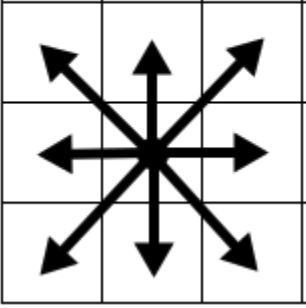
\includegraphics[scale=0.5]{pics/richtungen.png}
    \caption{Mögliche Richtungsentscheidungen der Clients mit dem jeweiligen Ausgangspunkt des Clients im mittleren Quadrat.}
    \label{fig:richtungen}
\end{figure}
%Grundlagen-Kapitel für KI
%Was ist KI? Welche Ansätze gibt es?

\subsection{Graphen}
Ein Graph wird definiert als eine Menge von Knoten und Kanten sowie deren Struktur und Anordnung.
Aus der Spezifikation der Map unseres Rennspiels lässt sich ein ungerichteter Graph mit 30x20 Knoten erstellen (siehe \autoref{fig:graphMaschen}).\newline

Maschen?\newline
Auch diagonal verbunden.\newline
Alle Spielknoten werden zunächst initial erzeugt.
Diese Spielknoten können anschließend mit Kanten verbunden werden (siehe \autoref{fig:graphMaschen}), und dienen als Grundlage für die im Folgenden genauer betrachteten Graph-Algorithmen und deren Funktionsweisen.\newline
Jeder einzelne Spielknoten repräsentiert dabei ein sog. \textit{Tile} (eine Kachel) der Map und kann folglich ein Segment der Strecke, ein Teil der Steinmauer (innen wie außen), ein Abschnitt der Wasserfläche oder auch die Start- und Zielflagge sein (siehe \autoref{fig:layout-mapeditor}).\newline
Bis auf die Eckspielknoten und die Spielknoten die am äußeren Rand der Karte liegen, besitzt jeder Knoten 8 Nachbarknoten, diesen umgebend.
Man kann also davon Sprechen, dass der Spielgraph ein 2-dimensionales Gitter darstellt, welches in x- und y-Richtung aufgespannt und anschließend über die Karte gelegt wird.
Während der Fortbewegung auf zwei in einer Reihe/Spalte nebeneinander liegenden Knoten, werden Kosten von 1 verursacht. Bei diagonaler Bewegung (bsp.: \textit{oben+links}) betragen die Kosten $\sqrt{2}$.
\begin{figure}[h]
    \centering
    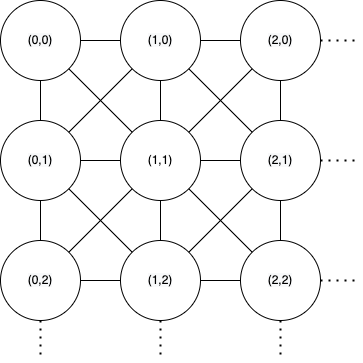
\includegraphics[scale=0.5]{pics/graph_maschen.png}
    \caption{Auschschnitt des Spielgraphen vom linken oberen \textit{Koordinatenursprung(0,0)} ausgehend.}
    \label{fig:graphMaschen}
\end{figure}


\subsection{Graph-Algorithmen}
Ein \textbf{Shortest-Path-Algorithmus} soll den kürzesten Weg zwischen zwei Punkten in einem Graphen finden. \textit{Short} meint in diesem Kontext nicht zwingend die physische Distanz, sondern kann sich auch auf Zeit, andere Kosten oder eine Kombination dieser Faktoren beziehen.\newline  
Zu den bekanntesten Shortest-Path-Algorithmen zählen die Algorithmen von \textit{Dijsktra}, \textit{Bellman-Ford}, \textit{Floyd-Warhsall}, sowie der \textit{A*}-Algorithmus.\newline
Pathfinding wird darüber hinaus auch verwendet, um einen gangbaren Weg durch eine Umgebung mit Hindernissen zu finden.


Für unser Rennspiel werden die Algorithmen von Dijkstra, sowie der A*-Algorithmus jeweils für einen KI-Client realisiert. Deren Implementierungen werden im später folgenden Abschnitt ... noch genauer beleuchtet. Zunächst soll allerdings noch die grundsätzliche Funktionsweise der Graphalgorithmen erläutert werden.\newline

\subsubsection{Dijkstra-Algorithmus}
Der Algorithmus von Dijkstra wurde bereits 1956 vom niederländischen Informatiker Edsger W. Dijkstra als optimaler Wegfindealgorithmus für Graphen entwickelt \cite{}.\newline
Die ursprüngliche Implementierung des Algorithmus lief im schlechtesten Fall mit einer Laufzeit von O(N2), wobei N die Anzahl der Knoten im Graphen ist.
Schnellere Implementierungen wurden später im Jahr 1984 von Fredman und Tarjan \cite{Fredman.1984} forgestellt, die im schlimmsten Fall eine Laufzeit von O(E + N log N) erreichen, wobei E die Anzahl der Kanten im Graphen ist.
Neben dem Graphen, benötigt der Algorithmus noch einen Start- und Zielknoten als Input. Sich dem Breitensuch-Algorithmus ähnelnd, schreitet er vom Startknoten aus in alle Richtungen voran.
Sobald der Zielknoten erreicht ist, kann der kürzeste Weg zum Startknoten zurückgerechnet werden.\newline
Während dem Suchvorgang werden die Knoten unterschieden zwischen \textit{gesehenen} und \textit{Grenzknoten}.\newline
Priority Queue\newline 
Ein zentrales Element des Algorithmus ist der sog. G-Wert, welcher ebenfalls jedem Knoten zugewiesen wird.
Bereits erforschte Knoten haben einen G-Wert gleich der Länge des kürzesten Weges zurück zum Startknoten. Für Knoten in der Grenzmenge ist er nur eine vorläufige Schätzung. Für Knoten, die nicht in diesen Mengen enthalten sind, ist der Wert undefiniert.\newline


 

\subsubsection{A*-Algorithmus}
Der A* (A-Stern) Algorithmus wurde zum ersten mal 1968 von einer Gruppe von Forschern des Stanford Research Institute vorgestellt \cite{aStern}. 
Dabei handelt es sich im Grunde um eine Erweiterung des Algorithmus von Dijsktra, indem versucht wird die Laufzeit durch die Einführung von Heuristiken zu optimieren.\newline
A* nutzt die Tatsache, dass alle Knoten räumliche Koordinaten haben. Diese Koordinaten können verwendet werden, um mit Hilfe einer Abstandsfunktion zu messen, wie weit ein Knoten vom Zielknoten entfernt ist.\newline

%Verwendete KI-Algorithmen erklären.


\subsection{OpenGL und Java-Swing}

Ein Ziel dieses Projektes ist es, das bereits vorhandene Grafikframework Java-Swing durch das Grafikframework OpenGL zu ersetzten. Der Hauptgrund für diese Entscheidung ist, dass die Java-Swing-Bibliothek nicht dafür ausgelegt ist ein Computerspiel effizient zu zeichnen. Mit OpenGL als ein Grafikframework, dass für die Computerspielanzeigt designt wurde, sodass eine Darstellung in Echtzeit von 2D-  und 3D-Grafikanwendungen möglich ist.

\subsubsection{LWJGL - Bibliothek}

Die Lightweight Java Game Library (LWJGL) ist eine Java-Computerspiel-Bibliothek, die eine plattformübergreifenden Zugriff auf verschiedene Schnittstellen ermöglicht. Für dieses Projekt wird die Bibliothek benötigt, um einen Zugriff auf OpenGL-Funktionen zu erhalten. Diese werden benötigt, da eine Grafik-Anwendung erstellt werden soll. Mit OpenGL ist es nicht möglich ein Spielfenster zu erstellen, um die Unabhängikeiten von Programmiersprache und Betriebsstyem zu erfüllten. Diesen Funktionalität übernehmen eingebundene Bibliotheken (wie GLFW) , die in der LWJGL Bibliothek includiert sind. Außerdem können somit umgebungsunabhängige Tastertur- und Mauseingaben erkannt werden.

\subsubsection{OpenGL - Definition}

OpenGL (OpenSource Grafics Library) ist eine Grafik-Schnittstelle, die genutzt werden kann um schnelle, bewegte 3D-Grafikbilder zu erstellen und zu manipuliere. Aber sie benötigt eine Programmiersprache in der es agieren kann. Ursprünglich wurde OpenGL für die Sprache C++ entwickelt. Da dieses Projekt in Java entwickelt wurden, wird die LWJGWL- Bibliothek (später Kapitel) benötigt, um OpenGL in Java nutzen zu können.
Ein großer Vorteil von OpenGL ist es betriebsystem und hardware-unabhängig zu sein, sodass auf OpenGL auf verschiedenen Betriebssystemen lauffähig ist. Das wurde auch in diesem Projekt getestet, denn für die Entwicklung wurde das Programm auf Linux, Window und einem OS-betriebenden Computer ausgeführt.

Das Einbinden der OpenGL-Bibliothek in das Projekt, wird mit der Maven-Configuration geregelt, sodass auch alle Abhängigkeiten berücksichtigt werden. 

In der OpenGL Spezifikation wird nur die Ausgabe definiert, was eine Funktion genau als Rückgabe liefert und wie genau sie funktionieren muss. Das erlaubt den Entwicklern beim Implementieren verschiedene Lösungen für Funktionsweise der Methoden zu finden. Deswegen gibt es in der OpenGL Spezifikation gibt keine Informationen über die Implementierung. In der Regel sind die Entwickler Grafikkarten-Hersteller, wo in der Hardware die Versionsuntertützung von OpenGL festgelegt wird.

\chapter*{OpenGL - Definition Grundlagen}

OpenGL hat zwei grundlegende Modi definiert. Der alte direkte Modus, zeichnete sich dadurch aus, das es eine Pipeline mit festen Funktionen gab. Diese Funktionen waren sehr einfach zu verwenden und man war in der Lage unmittelbar Grafiken zu zeichnen. Der große Nachteil dieser Funktionen bestand darin, dass die Entwickler keine Kontrolle darüber besaßen, wie OpenGL seine Berechnungen durchführte. 

Der neue OpenGL Ansatz wird als OpenGL-Core-Profil bezeichnet und wurde mit OpenGL Version 3.3 eingeführt. Dort wird man von OpenGL gedrängt die modernen Praktiken zu verwenden, indem OpenGL Fehler meldet und das Zeichnen der Grafik einstellt. Der moderne Ansatz hat den Vorteil sehr flexibel und effizient zu sein, denn die können genauer kontrollieren was genau und wann etwas gezeichnet wird. Der große Nachteil dieses Modus ist, das ein Entwickler die Grafikprogrammierung wirklich verstehen muss, um sie überhaupt anzuwenden.

In diesem Projekt wird der neue OpenGL-Core-Profil Ansatz verwendet, da der Hauptgrund eines Frameworkwechsels darin bestand, die Berechnung der Grafikkomponente dieses Rennspielframeworks effizienter zu gestalten.

Eine der Kernprinzipien nach der OpenGL arbeitet ist, dass OpenGL eine Status Maschine ist. Eine bestimmte Anzahl an Variablen definiert wie OpenGL im Augenblick arbeiten soll. Erst mit mit änderen bestimmter Variablen wird der Status der Anzeige geändert, sodass anstadt Dreiecke zum Beispiel Linien gezeichnet werden.

Zu berücksichtigen ist bei OpenGL das die Bibliothek in C geschrieben wurde. Deswegen sind in OpenGL viele Funktionalitäten, auch wenn eine andere Programmiersprache wie Java genutz wird, der von C sehr ähnlich. So muss auch in einem Java Programm Speicherplatz angefordert werden und es müssen spezielle Konstrukte verwendet werden, wie zum Beispiel Objekte die einem C struct entsprechen.

\subsubsection{Die Grafikpipeline in OpenGL}

OpenGL ist definiert, das sich jedes Spielobjekt in einem dreidimensionalen Raum befindet. Das Problem mit dem man konfrontiert wird ist, dass am Ende die Grafik auf einem 2D-Spielfenster angezeigt werden muss. OpenGL hat die meiste Arbeit damit 3D-Koordinaten in ein 2D-Array von Pixeln zu konvertieren, die Prozess wird in OpenGL mit einer Grafik-Pipeline verwaltet. Dieser Umwandlungsprozess geschieht in zwei Teilen. Beim ersten Teil werden die 3D-Koordinaten in 2D-Koordinaten umgewandelt und beim zweiten Teil werden diese 2D-Koordinaten zu farbigen Pixel übersetzt.

Die Grafikpipeline wird in mehrere Schritte unterteilt, wobei die Eingabe jedes Schrittes die Ausgabe des vorherigen Schrittes erfordert. Diese schritte haben immer nur eine bestimmte Aufgabe und können parallel ausgeführt werden. Aufgrund der Internen Struktur einer Grafikkarte mit vielen kleinen Rechenkernen können die Daten sehr schnell verarbeitet werden. Die Programme die diese Rechenschritte ausführen werden Shader genannt.

Ein paar dieser Shader sind indivduell an die eigenen Anwendung anpassbar, sodass eigene Shader entwickelt werden können. Dadurch besitzt man eine viel genauere Kontrolle über die Grafikpipeline und man kann mit diesen CPU-Zeit einsparen, da die aufwendige Berechnungen auf die GPU ausgelagert werden. Die Shader werden in einer für OpenGL entwickelten Programmiersprache geschrieben der OpenGL Shading Language (GLSL).

%Bild

In der gezeigten Grafik sieht man die abstrakte Darstellung von den Prozessen in der Grafik-Pipeline. Dort kann man sehen wie in einzelnen Schritten aus 3D-Koordinaten, die Vertex-Daten bezeichnet werden, in einzelnen Schritten zeichenbare Pixels entstehen. Der Vertex-, Geometry- und Fragment Shader können durch eigene Shader ausgetauscht werden. Ein Vertex ist ein Sammlung von Eigenschaften eines Punktes, das können Postionsdaten, Farbwerte, Texturen sein.

\chapter*{Shaders in der Grafikpipeline}

Der erste Teil der Pipeline ist der Vertex-Shader, dort wird ein einzelner Vertex eingegeben. Seine Aufgabe ist es eine 3D Koordinate in eine andere 3D Koordinate umzuwandeln. Der Vertex-Shader ermöglicht es grundlegende Verarbeitungen an den Vertex-Eigenschaften vorzunehmen. %%noch mehr

Die Primitiv-Assembly-Phase nimmt die vom Vertex-Shader zurückgelieferten Vertexe und setzt sie zu einer einfachen Form zusammen. Das können Linien, Rechtecke oder auch Dreiecke sein.

Alle ausgebenen primitiven Formen werden als nächstes im Geometrieshader bearbeitet. Dort werden andere oder zusätzliche Vertex-Punkte erstellt mit denen neue Formen/Primitive gebildet werden.

In der Rasterisierung werden alle Formen die im Geometrieshader entstehen, werden auf die entsprechenden Pixel des Bildschirms aufgeteilt. Das führt zu Fragmenten, die der Fragmentshader verwendet. Davor wird aber noch ein Clipping durchgeführt, das alle Fragmente entfernt die sich außerhalb der Ansicht befinden um die Leistung zu erhöhen.

Die wichtigste Aufgabe nämlich vom einfärben der Pixel übernimmt der Fragment-Shader. In diesem Schritt können fortgeschrittene OpenGL-Effekte, wie flackern, Nebel usw. eingefügt werden. In der Regel werden hier Standdardeffekte eingefügt, wie Schatten, Licht und dessen Farbe.

Nach der Ermittlung der Farbwerte kommt noch eine sogennante Alphatest- und Überblendungsphase. Da man sich im dreidimensionalen Raum befindet, werden hier Tiefenwerte der Fragmente überprüft. Wenn sich Objekte überdecken werden diese entsprechend verworfen. Auch werden hier die Alphawerte (diese definieren die Deckkraft eines Objektes überprüft.

Der ganze Prozess der Grafikpipeline ist ein ziemliches komplexes Gerüst, das aber die Möglichkeit gibt vieles selbst zu konfigurieren. Der Vertex- und Fragment-Shader werden in diesem Projekt selbst definiert, da auf der GPU keine Standdard-Shader exisitieren.





\subsubsection{ImGUI}

Um den Quellcode so effizient wie möglich zu gestalten, werden für die Implementierung Entwurfsmuster verwendet. Im Folgenden werden die verwendeten Muster erläutert, um für eine gute Grundlage zu sorgen. Die Umsetzung dieser Muster werden in den jeweiligen Kapiteln weiter ausgeführt.
\\
Um weitere Grundlagen für das kommende Implementier-Kapitel zu schaffen, werden zuvor die verwendeten Entwurfsmuster erläutert. Zusätzliche werden hierbei auf Vor- und Nachteile eingegangen.
\subsection{Entwurfsmuster}
Zuerst wird das Memento-Muster behandelt. Anschließend folgen Strategie und Template.

%Verwendete Entwurfsmuster für das HSP erklären.
%Vergleich zu anderen ähnlichen Mustern und begründen.
\subsubsection{Memento}
Die Motivation des \textit{Memento}-Musters ist laut \cite[S. 283 ff.]{gamma.2011} das Zurücksetzen eines Zustands ohne hierbei interne Eigenschaften der Klassen preiszugeben. 
\begin{figure}[h]
\centering
\begin{tikzpicture}
\tikzumlset{fill class = white, fill template = white}
	\umlclass[x=0]{Originator}{ - Zustand }{ + SetZustand(m : Memento)\\ + ErzeugeMemento() }
	\umlclass[x=6]{Memento} { - Zustand }{ + GetZustand()\\ + SetZustand() }
	\umlclass [x=11.5] {Caretaker}{}{}

	
	\umlimport[]{Originator}{Memento};
	\umluniaggreg[arg=memento, pos=0.5]{Caretaker}{Memento};
	%\umlnote[y=-3, width=4cm, fill=white]{Kontext}{ruft auf:\\ strategie.algorithmus()}

\end{tikzpicture}
\caption{Memento-Muster \cite[In Anlehnung an][S.285]{gamma.2011}}
\label{fig:memento_pattern}
\end{figure}

Das Verhaltensmuster besteht aus den in \autoref{fig:memento_pattern} dargestellten Elementen:
\begin{itemize}
\item \texttt{Originator}: Stellt einen Zustand dar, welcher in einem \texttt{Memento}-Objekt gespeichert werden kann.
\item \texttt{Memento}: Hier wird das \texttt{Originator}-Objekt in Form eines Zustands gespeichert. 
\item \texttt{Caretaker}: Verwaltet die bereits erzeugten \texttt{Mementos}, greift aber nicht auf den Inhalt der Zustände zu. Dieses Element ist also dafür zuständig, beliebige Zustände wiederherzustellen.
\end{itemize}
Das Memento-Muster bringt zudem folgende Konsequenzen mit sich:
\begin{itemize}
\item Das Muster schirmt andere Objekte von potenziell komplexen Originator-Interna ab und bewahrt so die Kapselungsgrenzen. Dies erfolgt dadurch, dass die Offenlegung von Informationen, die nur von einem Originator verwaltet werden sollten, die aber dennoch außerhalb des Originators gespeichert werden müssen, vermieden werden.
\item Da die gesamte Speicherverwaltung nicht beim \texttt{Originator} liegt, vereinfacht die Verwaltung des angeforderten Zustands den \texttt{Originator}.
\item Wenn der \texttt{Originator} eine große Menge an Informationen kopieren muss, um einen \texttt{Memento} zu erzeugen, wird hier ein Overhead verursacht. Das bedeutet also, wenn die Wiederherstellung des \texttt{Originator}-Zustands sehr aufwändig ist, ist das Memento-Muster infolgedessen auch sehr aufwändig.
\item Da die \texttt{Caretaker}-Instanz keine Information darüber hat, wie viele Daten in einem \texttt{Memento} enthalten sind, kann ein Speichern der \texttt{Memento}-Instanzen große Speicherkosten verursachen.
\end{itemize}




\subsubsection{Strategie}
Das \textit{Strategie}-Muster wird dafür verwendet, falls es verwandet Klassen gibt, die sich in dessen Verhalten unterscheiden. Dieses Verhaltensmuster wird also eingesetzt, falls beispielsweise viele Algorithmen verwaltet werden sollen. Es wird hierbei auf die Algorithmen über eine zentrale Instanz zugegriffen.\\
Es treten hier folgen Elemente auf, welche in \autoref{abb:strategy} zu sehen sind, wobei die Erklärung der Komponenten zunächst verallgemeinert und anschließend anhand des Algorithmen-Beispiels verdeutlicht wird:
\begin{itemize}
\item \texttt{A-Strategie}: Diese abstrakte Klasse dient der Beschreibung der Methoden, die die Unterklassen besitzen sollen. Im Falle mehrerer Algorithmen könnte dies der Start besagter Algorithmen sein.
\item \texttt{KonkreteStrategie}: Hier werden beispielsweise die verschiedenen Algorithmen im Detail implementiert. \texttt{KonkreteStrategieA} und \texttt{KonkreteStrategieB} können in diesem Fall die Funktionalitäten beinhalten, die über die \textbf{algorithmus}-Methode einen Start der konkreten Algorithmen hervorbringen könnte.
\item \texttt{Kontext}: Dieses Element entscheidet darüber, welche Instanz von \texttt{A-Strategie} dem Aufrufer geliefert werden soll. In diesem Beispiel könnte die Art des zu liefernden Algorithmus in einer Konfigurationsdatei angegeben werden, welche beim Aufruf der \textbf{operation}-Methode eingelesen wird. Abschließend bekommt der Aufrufer eine Instanz der gewünschten Komponente.
\end{itemize}  

\begin{figure}[h]
\centering
\begin{tikzpicture}
\tikzumlset{fill class = white, fill template = white}
	\umlinterface[x=8]{A-Strategie}{ }{\umlvirt{ + algorithmus() : void} }
	\umlclass[x=5,y=-3]{KonkreteStrategieA} { }{+ algorithmus() : void}
	\umlclass[x=11,y=-3]{KonkreteStrategieB} { }{+ algorithmus() : void}
	\umlclass{Kontext}{} {+ operation() : void}
	
	\umlinherit{KonkreteStrategieA}{A-Strategie}
	\umlinherit{KonkreteStrategieB}{A-Strategie}
	\umlaggreg[arg=strategie, pos=0.5]{Kontext}{A-Strategie}
	\umlnote[y=-3, width=4cm, fill=white]{Kontext}{ruft auf:\\ strategie.algorithmus()}

\end{tikzpicture}
\caption{Strategie-Muster \cite{Goll.2014}}
\label{abb:strategy}
\end{figure}

Dieses Muster besitzt die folgenden Vorteile:\\
\begin{itemize}
\item Es wird aufgrund der Kapselung der \texttt{KonkretenStrategien} für eine Erleichterung der Erweiterung und Umstellung gesorgt.
\item Es können bedingte Anweisungen im Quellcode reduziert werden, da nun jede \texttt{Konkrete-Stategie} eine eigene Klasse darstellt.
\item Darauf folgend können die gemeinsamen Funktionalitäten der \texttt{KonkretenStrategien} herausarbeitet werden.
\end{itemize}
Eine negative Eigenschaft dieses Musters, ist der Kommunikations-Overhead zwischen den Instanzen \texttt{Kontext} und \texttt{A-Strategie}. Falls  beispielsweise \texttt{KonkreteStrategieA} und \texttt{Konkrete-StrategieB} unterschiedliche Informationen zum Erzeugen deren Instanzen benötigen, z.B. benötigt eine Klasse nur eine Anzahl an Iterationsschritten, wohingegen die andere Komponente zusätzlich mehrere Flags benötigt. In diesem Fall ist eine engere Kopplung zwischen \texttt{Kontext} und \texttt{A-Strategie} notwendig \cite[S. 315 ff.]{gamma.2011}.\\
Ähnlich zum Strategie-Muster gibt es das Template-Muster, welches im Folgenden weiter erläutert wird. Zusätzlich werden das Strategie- und Template-Muster verglichen.
\subsubsection{Template-Muster}
Dieses Verhaltensmuster wird laut \cite[325ff.]{gamma.2011} dafür eingesetzt, wenn es beispielsweise einen Algorithmus gibt, der sich zu einem anderen Algorithmus nur an wenigen Stellen des Ablaufs unterscheidet.\\
\begin{figure}[h]
\centering
\begin{tikzpicture}
\tikzumlset{fill class = white, fill template = white}
	\umlclass[x=6,type=abstract]{AbstrakteKlasse}{ }{ + TemplateMethode()\\ + \umlvirt{ Operation1() }\\ + \umlvirt{ Operation2()} }
	\umlclass[x=0]{KonkreteKlasse} { }{ + Operation1()\\ + Operation2() }
	\umlnote [x=11, fill=white] {AbstrakteKlasse}{ ...\\ Operation1()\\ ...\\ Operation2()\\ ...}

	
	\umlinherit{KonkreteKlasse}{AbstrakteKlasse}
	%\umlnote[y=-3, width=4cm, fill=white]{Kontext}{ruft auf:\\ strategie.algorithmus()}

\end{tikzpicture}
\caption{Memento-Muster \cite[In Anlehnung an][S.327]{gamma.2011}}
\label{fig:template}
\end{figure}
Wie in \autoref{fig:template} zu sehen ist, besteht dieses Muster aus den zwei Komponenten \texttt{AbstrakteKlasse} und \texttt{KonkreteKlasse}.\\
Die \texttt{AbstrakteKlasse} beschreibt hierbei einen Algorithmus mit der \textbf{TemplateMethode}, welche die abstrakten Operationen \textbf{Operation1} und \textbf{Operation2} verwendet.\\
Die \texttt{KonkreteKlasse} überschreibt hierbei lediglich \textbf{Operation1} und \textbf{Operation2}.\\
Mithilfe dieses Mechanismus kann der Ablauf eines Algorithmus festgelegt und vorgegeben werden. Zusätzliche Algorithmen, die sich im Ablauf ähneln, aber an wenigen Stellen ein anderes Verhalten aufzeigen, können hier also leicht ergänzt werden.\\
Im Folgenden werden sowohl das Template-Muster, als auch das Strategie-Muster verglichen, da für dieses Projekt mehrere Algorithmen eingesetzt werden und somit ein Mechanismus notwendig ist, diese so einfach wie möglich verwalten zu können.\\
Wie bereits beschrieben, hilft Template dabei den Ablauf eines Algorithmus festzulegen. Allerdings fehlt hierbei ein Mechanismus, der dabei hilft zwischen mehreren Algorithmen einen beliebigen auszuwählen. Dies ermöglicht Strategie mithilfe der \texttt{Kontext}-Klasse. Dazu folgt, dass bei Algorithmen, die sich im Ablauf komplett unterscheiden Template nicht hilfreich ist und hier Strategie mehr Möglichkeiten bringt.\\
Falls es also mehrere Algorithmen gibt, die sich nur an wenigen Stellen im Ablauf unterscheiden, so ist eine Kombination beider Verhaltensmuster eine Möglichkeit, den Ablauf vorzugeben und eine \texttt{Kontext}-Klasse anzubieten, die dem Nutzer eine Instanz des jeweiligen Algorithmus liefert.

Da nun die Grundlagen zum Verständnis vermittelt wurden, wird im Folgenden auf den Hauptteil dieses Berichts eingegangen, die Implementierung. 
\pagebreak

\section{Implementierung}

\subsection{Der Map-Editor}
Ein weiteres Ziel dieses Projekts ist das Implementieren einer Applikation, die das Entwerfen und Speichern der Spielfelder, inklusive Checkpunkte und Startpositionen, erleichtern soll. Diese Applikation wird im Folgenden als Map-Editor bezeichnet.\\
In diesem Kapitel wird zunächst das Vorgehen der Erstellung eines Spielfeldes im Ausgangszustand des Rennspielframeworks geschildert. Anschließend wird auf das Konzept des Map-Editor eingegangen. Abschließend wird die Implementierung der Komponenten erläutert.\\

\subsubsection{Vorheriges Vorgehen bei der Spielfeld-Erstellung}
Da die Spielfelder mit ASCII-Zeichen kodiert werden und das Spielfeld hinzukommend eine festgelegte Größe von 20x30 Kacheln hat, ist das händische Erstellen einer solchen Datei ein aufwändiges Vorgehen. Hierbei besitzt jede Kachel eine eigene Identifikationsnummer. Ein Beispiel eines Spielfeldes und dessen Kodierung wird in \autoref{fig:simple_kodiert} dargestellt.\\

\begin{figure}[h]
\centering
\begin{minipage}{1.0\textwidth}
\centering
\begin{minipage}[t]{0.6\textwidth}
\centering
\begin{spacing}{1.0}
\fontsmall
MAP\\
10 10 10 10 10 10 10 10 10 10 10 10 10 10 10 10 10 10 10 10 10 10 10 10 10 10 10 10 10 10\\
10 20 20 20 20 20 20 20 20 20 20 20 20 20 20 20 20 20 20 20 20 20 20 20 20 20 20 20 20 10\\
10 20 21 18 18 18 18 18 18 18 18 18 18 18 18 18 18 18 18 18 18 18 18 18 18 18 18 22 20 10\\
10 20 16 11 11 11 11 11 11 11 11 11 11 11 11 11 11 11 11 11 11 11 11 11 11 11 11 15 20 10\\
10 20 16 11 11 11 11 11 11 11 11 11 11 11 11 11 11 11 11 11 11 11 11 11 11 11 11 15 20 10\\
10 20 16 11 11 12 13 13 13 13 13 13 13 13 13 13 13 13 13 13 13 13 13 13 14 11 11 15 20 10\\
10 20 16 11 11 15 20 20 20 20 20 20 20 20 20 20 20 20 20 20 20 20 20 20 16 11 11 15 20 10\\
10 20 16 11 11 15 20 20 20 20 20 20 20 20 20 20 20 20 20 20 20 20 20 20 16 11 11 15 20 10\\
10 20 16 11 11 15 20 20 20 20 20 20 31 32 32 32 33 20 20 20 20 20 20 20 16 11 11 15 20 10\\
10 20 16 11 11 15 20 20 20 20 20 20 34 30 30 30 35 20 20 20 20 20 20 20 16 11 11 15 20 10\\
10 20 16 11 11 15 20 20 20 20 20 20 36 37 37 37 38 20 20 20 20 20 20 20 16 11 11 15 20 10\\
10 20 16 11 11 15 20 20 20 20 20 20 20 20 20 20 20 20 20 20 20 20 20 20 16 11 11 15 20 10\\
10 20 16 11 11 15 20 20 20 20 20 20 20 20 20 20 20 20 20 20 20 20 20 20 16 11 11 15 20 10\\
10 20 16 11 11 15 20 20 20 20 20 20 20 20 20 20 20 20 20 20 20 20 20 20 16 11 11 15 20 10\\
10 20 16 11 11 17 18 18 18 46 18 18 18 18 18 18 18 18 18 18 18 18 18 18 19 11 11 15 20 10\\
10 20 16 11 11 11 11 11 11 45 09 09 11 11 11 11 11 11 11 11 11 11 11 11 11 11 11 15 20 10\\
10 20 16 11 11 11 11 11 11 45 09 09 11 11 11 11 11 11 11 11 11 11 11 11 11 11 11 15 20 10\\
10 20 23 13 13 13 13 13 13 47 13 13 13 13 13 13 13 13 13 13 13 13 13 13 13 13 13 24 20 10\\
10 20 20 20 20 20 20 20 20 20 20 20 20 20 20 20 20 20 20 20 20 20 20 20 20 20 20 20 20 10\\
10 10 10 10 10 10 10 10 10 10 10 10 10 10 10 10 10 10 10 10 10 10 10 10 10 10 10 10 10 10\\
\fontnormal
\end{spacing}
\label{fig:map_in_ascii}
\end{minipage}
\qquad
\begin{minipage}[t]{0.2\textwidth}
\begin{spacing}{1.0}
\fontsmall
CHECKPOINT\\
07 16 01\\
07 17 01\\
04 14 02\\ 
05 14 02\\
04 07 03\\
05 07 03\\
08 04 04\\
08 05 04\\
23 04 05\\
23 05 05\\
26 08 06\\
27 08 06\\
26 14 07\\
27 14 07\\
STARTPOINT\\
10 15 3\\
10 16 3\\
11 15 3\\
 11 16 3\\


\end{spacing}
\fontnormal
%\subcaption{Kodierung der Check- und Startpositionen}
\end{minipage}
\subcaption{Kodierung des Spielfeldes mit Checkpunkten und Startpositionen}
\end{minipage}
\begin{minipage} {0.9\textwidth}
\centering
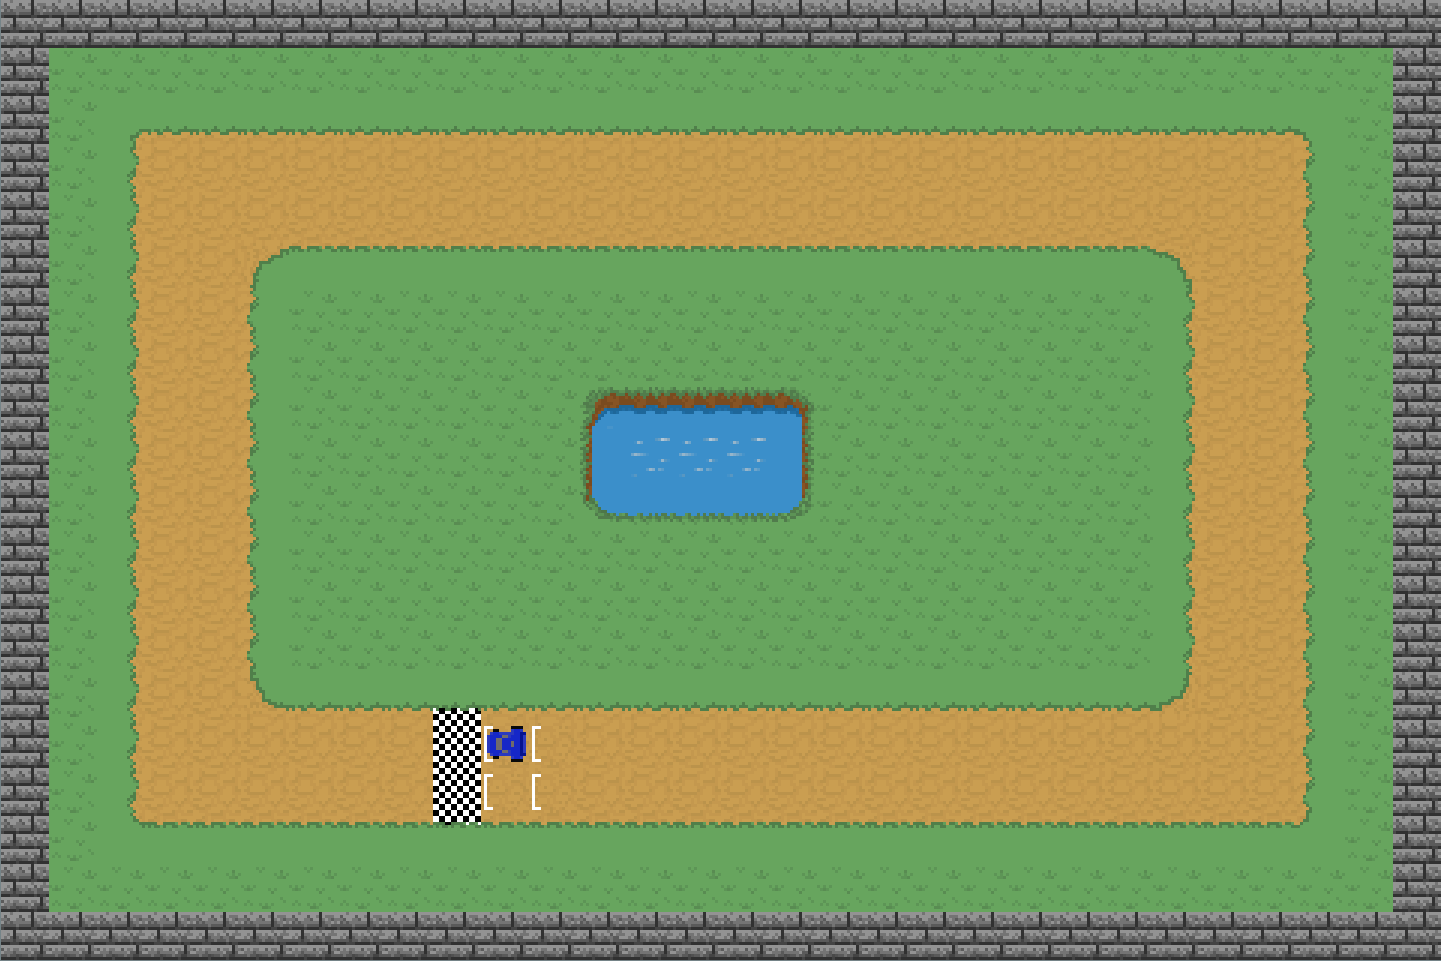
\includegraphics[scale=0.25]{pics/simples_spielfeld.png}
\label{fig:check_start}
\subcaption{Ergebnis der obigen Kodierung}
\end{minipage}
\caption{Beispielhaftes Spielfeld mit der dazugehörigen Kodierung}
\label{fig:simple_kodiert}
\end{figure}

Hinzukommend müssen die Positionen für die Start- und Checkpunkte (siehe \autoref{fig:check_start}) angegeben werden. Damit diese und weitere Informationen für ein Spiel verwendet werden können, müssen diese in einer JSON-Konfigurationsdatei abschließend angegeben werden. Anhand dieses Beispiels ist gut zu erkennen, dass das Erstellen eines Spielfeldes einen aufwändigen Prozess darstellen kann.\\
Der Map-Editor soll dementsprechend folgende Anforderungen erfüllen:
\begin{itemize}
\item Das Erstellen des Spielfeldes soll dem Nutzer nicht nur via ASCII-Kodierung gelingen können.
\item Der Nutzer soll dazu in der Lage sein, Start- und Checkpunkte setzen zu können.
\item Das Spielfeld, dessen Start- und Checkpunkte sollen anschließend korrekt kodiert in einer Datei gespeichert werden.
\end{itemize}
Um die Umsetzung dieses Vorgehens und die Erweiterung neuer Funktionalitäten dem Entwickler zu erleichtern, orientiert sich die Architektur des Map-Editors an dem MVC-Architekturmuster (siehe Kapitel ???). Die Umsetzung der Architektur wird im folgenden Abschnitt genauer erläutert.

\subsubsection{Architektur des Map-Editors}
In der folgenden Abbildung werden die grundlegenden Komponenten des Editors in Form eines Domänenmodells dargestellt.\\

\begin{figure}[h]
\centering
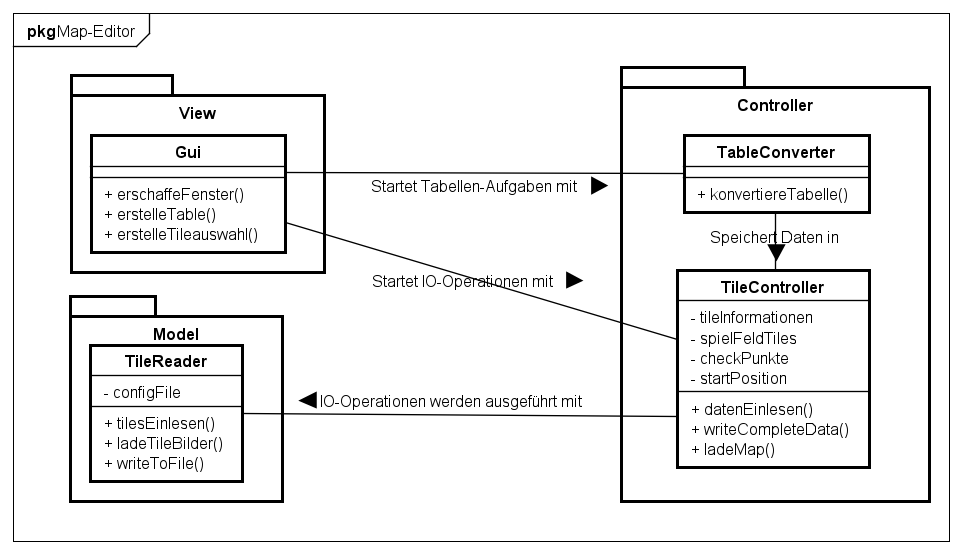
\includegraphics[scale=0.5]{pics/mapeditor_domain.png}
\caption{Domänenmodell des Map-Editors}
\label{fig:domain_mapeditor}
\end{figure}

Das MVC-Muster ist hierbei wie folgt zu sehen:
\begin{itemize}
\item View wird durch die \texttt{GUI}-Komponenten dargestellt. Alle Aufgaben, die zur Ausgabe dienen, sind vereinfacht in dieser Komponente zusammengefasst. Der Übersichtlichkeit halber werden hier nicht alle Komponenten, die mit der Aktion des Anwenders zu tun haben dargestellt.
\item Controller wird durch die Komponenten \texttt{TileController} und \texttt{TableConverter} dargestellt. Zusätzlich befinden sich hier die Komponenten des Memento-Entwurfsmusters. Diese Komponenten werden der Einfachheit halber nicht dargestellt. Eine nähere Erläuterung der Umsetzung dieses Musters erfolgt im kommenden Abschnitt.
\item Model wird durch \texttt{TileReader} dargestellt. Diese Komponente übernimmt alle E/A-Aufgaben, wozu das Einlesen und Erstellen von Konfigurationsdateien des Spielfeldes zählen.
\end{itemize}
Dieses Architekturmuster hilft hierbei eine eindeutige Trennung der Komponenten und deren Funktionalität zu schaffen. Wird nun beispielsweise aus der \texttt{Gui} das Speichern des aktuellen Spielfeldes gestartet, so erfolgt eine Verbindung zur Model-Schicht mittels des \texttt{TileControllers}, damit für eine zusätzliche klare Trennung der Schichten gesorgt werden kann. Dementsprechend fungiert der \texttt{TileController} als Hauptansprechpartner, falls eine Aktion aus der \texttt{Gui} heraus gestartet wird. Dies bringt zwar eine niedrige Kohäsion mit sich, da die \textit{TileController}-Komponente für sowohl das Speichern von Dateien, als auch für das Ausführen der Logik der \textit{Gui}-Aktionen zuständig ist. Dies hat jedoch bei den überschaubaren Funktionalitäten des Map-Editors, die im kommenden Abschnitt genauer beschrieben werden, eine geringe Auswirkung.\\
Die Implementierung der Komponenten und zusätzliche Eigenschaften des Map-Editors werden im folgenden Unterabschnitt erläutert, wobei zunächst auf die Funktionalität und den Ablauf des Erstellen eines Spielfeldes eingegangen wird.

\subsubsection{Implementierung des Map-Editors}
Wie in \autoref{fig:layout-mapeditor} zu sehen ist, besteht die grafische Oberfläche des Map-Editors aus drei Label, in denen sich eine Auswahl möglicher Kacheln (links), das aktuelle Spielfeld in Form einer Tabelle (rechts oben) und eine Auswahl der möglichen Befehle, die der Nutzer zur Bearbeitung des Spielfelds verwenden kann, in Form von Buttons (unten).

\begin{figure} [h]
\centering
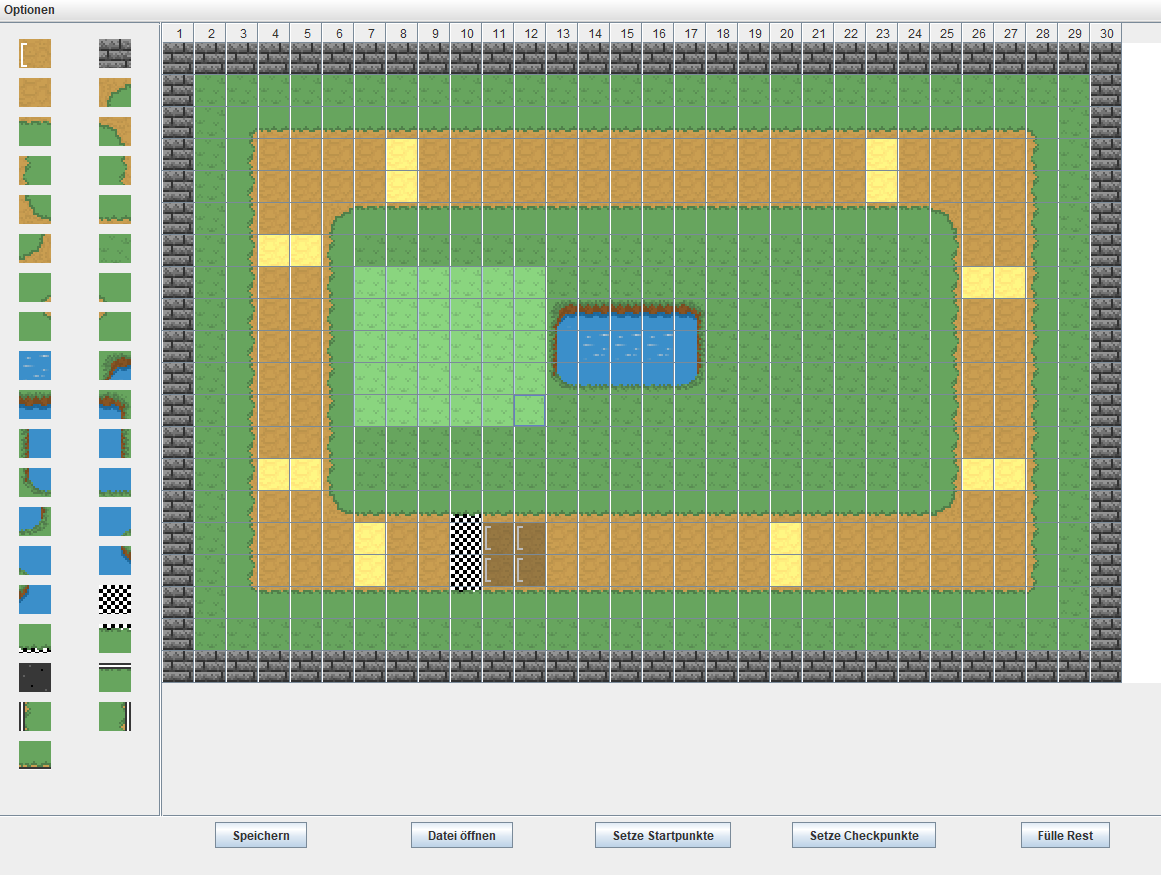
\includegraphics[scale=0.45]{pics/map-editor-layout.png}
\caption{Grafische Oberfläche des Map-Editors}
\label{fig:layout-mapeditor}
\end{figure}

Für die Auswahl möglicher Kacheln werden diese Daten aus einer Konfigurationsdatei erfasst. Diese Aufgabe übernimmt die Komponente \texttt{TileReader} aus der Model-Komponente. Es werden hierbei zuerst alle möglichen Kacheln mit deren IDs eingelesen. Anschließend werden die Bilder dieser Kacheln eingelesen. Jedes Kachelbild wird mit der korrespondierenden ID der Kachel in einem Label gespeichert. Anschließend wird nur das Bild als visuelle Ausgabe des Labels dargestellt. Jedes Label hat also das Kachel-Bild und die korrespondierende ID gespeichert. Die ID ist hierbei notwendig, um abschließend aus der Tabelle eine Konfigurationsdatei des Spielfeldes in ASCII-Form abspeichern zu können.\\
Die Tabelle rechts in \autoref{fig:layout-mapeditor} dient, wie bereits beschrieben, dem Erstellen der Spielfelder. Die Tabelle zeigt hierbei nur das Bild der Kachel an. Zusätzlich wird in jeder Zelle der Tabelle die dazugehörige ID zur Kachel abgespeichert, damit das Speichern des Spielfeldes zusätzlich erleichtert wird.\\
Was den Vorgang des Erstellen des Feldes betrifft, so soll der Anwender die gewünschte Kachel aus dem Auswahlmenü in die jeweilige Zelle der Tabelle ziehen. Falls mehrere Zellen auf einmal befüllt werden sollen, so kann ein Bereich markiert werden. Wird in diesem Bereich eine Kachel reingezogen, so wird der ausgewählte Bereich auf einmal überschrieben. Dies hat die Intention, dem Anwender das Erstellen der Spielfelder zu erleichtern und zusätzlich den gesamten Ablauf zu verkürzen. Der Rand des Spielfeldes wird hierbei standardsgemäß mit der Mauer-Kachel gefüllt und kann nicht von anderen Kacheln überschrieben werden. Dies ist notwendig, damit die Spieler nicht aus dem Spielfeld hinaus fahren können.\\
Sind Zellen noch nicht überschrieben worden, stellen diese also eine leere Zelle dar, so wird für diese Zellen die Kachel-ID -1 verwendet und ein weißes Bild zur Ausgabe verwendet. Stellt eine Zelle einen Start- oder Checkpunkt dar, so werden die Bilder dieser Zellen aufgehellt, um dem Anwender dies zu visualisieren.\\
Weitere Funktionalitäten des Map-Editors und deren Implementierung lauten wie folgt:

\textbf{Das Füllen aller leeren Zellen der Tabelle mit Grass}\\
Hierbei wird über den gesamten Tabelleninhalt iteriert und die Zellen, die aktuell noch mit der ID -1 gefüllt sind, mit den Grass-Tiles überschrieben. So kann sich der Anwender auf das Erstellen der Strukturen der Rennstrecken fokussieren und die Zeit zum Erstellen eines Spielfeldes wird zusätzlich reduziert.

\textbf{Das Erstellen von Startpositionen und Checkpunkten}\\
Hierfür muss mindestens eine Zelle der Tabelle ausgewählt sein. Der Nutzer wird anschließend nach der Positionierungsrichtung der Fahrzeuge gefragt. Die Koordinaten und die angegebene Richtung werden anschließend gespeichert. Werden neue Startpositionen ausgewählt, so werden diese standardsgemäß zu den aktuell gespeicherten Startpositionen hinzugefügt. Das Setzen der Checkpunkte erfolgt analog zu den Startpunkten, jedoch ohne der Auswahl der zu fahrenden Richtung der Spieler. Auch hier werden neu gesetzten Checkpunkte zu den aktuell gespeicherten Punkten hinzugefügt.

\textbf{Das Löschen der Start- und Checkpunkte}\\
Der Nutzer kann alle bereits gesetzten Startpunkte löschen. Hierbei werden lediglich die gespeicherten Startpunkte auf den Initialwert zurückgesetzt. Das Löschen aller Checkpunkte erfolgt hierzu erneut analog.

\textbf{Bereits erstellte Spielfelder einlesen}\\
Um bereits erstelle Spielfelder überarbeiten zu können, kann der Anwender die zu überarbeitende Datei in einem Auswahlmenü selektieren. Anschließend werden diese Datei eingelesen. Die Tabelle wird abschließend komplett überschrieben, so dass diese der eingelesenen Informationen ähnelt.

\textbf{Das Füllen eines Bereichs der Tabelle}\\
Wie bereits erwähnt, können mehrere Felder gleichzeitig befüllt werden. Hierzu kann der Nutzer einen beliebigen Bereich der Tabelle auswählen und anschließend eine beliebige Kachel auf eines der markierten Felder ziehen. Bei diesem Vorgang wird zunächst überprüft, ob mehrere Zellen ausgewählt wurden. Ist dies der Fall, so werden alle betroffenen Zellen überschrieben.

\textbf{Das Visualisieren des markierten Bereichs und der Start- und Checkpunkte}\\
Damit der markierte Bereich dem Anwender visuell dargestellt werden kann und der Anwender somit eine Rückmeldung des Programms bekommt, wird bei jedem Aktualisieren der Tabelle das Bild der markierten Zelle heller abgespeichert (siehe \autoref{fig:layout-mapeditor}). Ist eine Zelle nicht mehr markiert, so wird auf das originale Kachel-Bild zurückgesetzt. Dieser Mechanismus wird auch bei den Startpositionen und Checkpunkten verwendet, damit diese dem Anwender deutlich dargestellt werden können. Hierbei werden die Startpositionen dunkler und die Checkpunkte heller dargestellt, wie in \autoref{fig:layout-mapeditor} zu sehen ist.

\textbf{Die Grenzen des Spielfelds werden nie überschrieben}\\
Damit die Grenzen des Spielfeldes immer vorhanden sind, ist der Rand der Tabelle immer mit einer Mauer-Kachel belegt. Versucht der Anwender trotzdem eines dieser Felder zu überschreiben, so wird dieser Befehl ignoriert. Dem Nutzer wird anschließend eine Warnmeldung ausgegebene. Die Überprüfung, ob ein Rand-Element überschrieben wird, erfolgt auch bei einer Mehrfachauswahl von Tabellen-Zellen.

\textbf{Das Speichern des Spielfeldes}\\
Beim Speichern des Spielfeldes und der zugehörigen Informationen wird zunächst überprüft, ob alle Zellen der Tabelle mit bekannten Tile-IDs gefüllt sind, mindestens ein Chechpunkt und mindestens ein Startpunkt gesetzt sind. Ist mindestens eine dieser Bedingungen nicht erfüllt, so wird zunächst eine Warnung, dass der Stand des Spielfeldes noch kein akzeptiertes Feld darstellt, ausgegeben. Anschließend kann der Anwender entweder abbrechen oder den aktuellen Stand trotzdem speichern, falls lediglich ein Zwischenstand gesichert werden soll. Bei dem Erstellen der Datei des Spielfeldes wird über den Tabelleninhalt iteriert und die Kachel-IDs werden wie in \autoref{fig:check_start} zeilenweise angeordnet und in eine neue Datei geschrieben. Die Check- und Startpunkte werden in derselben Datei gespeichert. Damit eine eindeutige Unterscheidung der verschiedenen Sektionen erfolgen kann, wird in die vorherige Zeile des jeweiligen Abschnitts ein Name geschrieben, der die dazugehörige Komponente bezeichnet. Den Namen der produzierten Konfigurationsdatei hat der Anwender zu Beginn des Vorgangs angegeben.

\textbf{Gemachte Aktionen rückgängig machen}\\
Des Weiteren kann der Anwender seine zuletzt durchgeführten Aktionen rückgängig machen. Die Umsetzung hierbei erfolgt über das Memento-Muster \textbf{(siehe Kapitel ??)}. Hierbei wird für den aktuellen Zustand der Inhalt der Tabelle, die gesetzten Startpunkte und die gesetzten Checkpunkte verwendet. Ein Zustand wird als Memento gespeichert, sofern sich der Tabelleninhalt, die Start- oder Checkpunkte verändern. Wird nun ein vorheriger Zustand geladen, so werden auch diese Informationen komplett überschrieben und die Tabelle wird zur Visualisierung aktualisiert. Das Memento-Muster ist hierbei wie folgt umgesetzt:

\begin{figure}[h]
\centering
\begin{tikzpicture}
\tikzumlset{fill class = white, fill template = white}
	\umlclass[x=0]{Originator}{ - karte \\ - startpunkte \\ - checkpunkte \\ - letzterSicherungspunkt \\ - caretaker }{ + erstelleSicherung()\\ + undo() \\ + restore() \\ + setOriginatorZustand(ID) }
	\umlclass[x=5.5]{Memento} { - katze \\ - startpunkte \\ - checkpunkte }{ + SetZustand() }
	\umlclass [x=11.3] {Caretaker}{ - zustände \\ - mementoID}{ + speichereMemento() \\ + getMemento(ID)}

	
	\umlimport[]{Originator}{Memento};
	\umluniaggreg[arg=memento, pos=0.5]{Caretaker}{Memento};
	%\umlnote[y=-3, width=4cm, fill=white]{Kontext}{ruft auf:\\ strategie.algorithmus()}

\end{tikzpicture}
\caption{Umsetzung des Memento-Musters für den Map-Editor}
\label{fig:memento_imp}
\end{figure}

\begin{itemize}
\item Wie in \autoref{fig:memento_imp} zu sehen ist, besitzt die \textit{Memento-Klasse}, die die gespeicherten Zustände darstellt, Attribute für das Spielfeld, den Startpositionen und den Checkpunkten.
\item Der \textit{Originator}, der den aktuellen Zustand des Editors darstellt, besitzt zusätzlich den letzten Sicherungspunkt der vorherigen \textit{Memento}-Instanz.
\item Hinzukommend wird ein Verwalter, der \texttt{Caretaker}, für das Erstellen und Wiederherstellen der Zustände verwendet. Dieser hat alle erstellten \textit{Memento}-Instanzen mit einer ID in einer Hash-Map abgespeichert. Mit der Angabe der jeweiligen ID kann nun ein beliebiger Zustand wiederhergestellt werden. Dies ermöglicht auch in Zustände zu gelangen, die bereits erreicht wurden, falls der Anwender z.B. zu oft rückgängig gemacht hat und wieder ein paar Zustände nach vorne gelangen will. 
\end{itemize}
Wird nun die Tabelle verändert, so wird der aktuelle Zustand der Tabelle in den \texttt{Originator} geschrieben und zusätzlich ein Sicherungspunkt erstellt. Der \texttt{Originator} wird zusätzlich verändert, wenn ein Sicherungspunkt oder ein Startpunkt gesetzt wird. Setzt nun der Anwender einen vorherigen Stand zurück, so wird die jeweilige \texttt{Memento}-Instanz geladen und der Zustand des \texttt{Originators} überschrieben. Wie bereits beschrieben, hat anschließend der Nutzer die Möglichkeit wieder einen Zustand nach vorne zu springen. Hierbei ergibt sich der folgende Spezialfall:\\
Macht der Anwender seine Änderungen rückgängig und ändert die Tabelle, so soll dieser nicht mehr nach vorne springen können, da ansonsten die neue Änderung des Nutzers verloren gehen würde. Tritt also ein solcher Fall ein, so werden nach der Überschreibung des \texttt{Originators}, also beispielsweise nach Tabellenänderung, alle nachfolgenden \texttt{Memento}-Elemente gelöscht, damit keine Inkonsistenzen entstehen. \autoref{fig:memento_example} veranschaulicht diesen Mechanismus.\\ 

\begin{figure}[h]
\centering
\begin{minipage}[b]{0.3\textwidth}
\centering
\begin{tikzpicture}
        \node at (0,0) [rectangle,draw] (a1) {$1_{a}$};
        \node at (1,0) [rectangle,draw] (a2) {$2_{a}$};
        \node at (2,0) [rectangle,draw] (a3) {$3_{a}$};
        \node at (3,0) [rectangle,draw] (a4) {$4_{a}$};
        \draw[->] (a4.north) -- ++(0,0.5) -- ++(-1,0) -- (a3.north);
        \draw[->] (a3.north) -- ++(0,0.5) -- ++(-1,0) -- (a2.north);
        \draw[-,dashed] (a1) -- (a2);
        \draw[-,dashed] (a2) -- (a3);
        \draw[-,dashed] (a3) -- (a4);
\end{tikzpicture}
\subcaption{Zwei Aktionen rückgängig}
\label{fig:memento_zweinachhinten}
\end{minipage}
\qquad
\begin{minipage}[b]{0.3\textwidth}
\centering
\begin{tikzpicture}
        \node at (0,0) [rectangle,draw] (a1) {$1_{a}$};
        \node at (1,0) [rectangle,draw] (a2) {$2_{a}$};
        \node at (2,0) [rectangle,draw] (a3) {$3_{b}$};
        \node at (3,0) [rectangle,draw,dashed] (a4) {$4_{a}$};
        \draw[->] (a2.north) -- ++(0,0.5) -- ++(1,0) -- (a3.north);
        \draw[-,dashed] (a1) -- (a2);
        \draw[-,dashed] (a2) -- (a3);
\end{tikzpicture}
\subcaption{Neue Aktion durchführen}
\label{fig:memento_überschreiben}
\end{minipage}
\qquad
\begin{minipage}[b]{0.25\textwidth}
\centering
\begin{tikzpicture}
        \node at (0,0) [rectangle,draw] (a1) {$1_{a}$};
        \node at (1,0) [rectangle,draw] (a2) {$2_{a}$};
        \node at (2,0) [rectangle,draw] (a3) {$3_{b}$};
        \draw[-,dashed] (a1) -- (a2);
        \draw[-,dashed] (a2) -- (a3);
\end{tikzpicture}
\subcaption{Endergebnis}
\label{fig:memento_nachher}
\end{minipage}

\caption{Ablauf, wenn ein nicht aktueller Zustand überschrieben wird}
\label{fig:memento_example}
\end{figure}

Hier befindet sich der aktuelle Zustand des Systems bei $4_{a}$. Der Anwender macht die letzten zwei Aktionen rückgängig und gelangt in den Zustand $2_{a}$ (siehe \autoref{fig:memento_zweinachhinten}). Anschließend erfolgt eine Änderung durch den Nutzer, wodurch der Zustand $3_{a}$ durch $3_{b}$, welcher den neuen Zustand beinhaltet, überschrieben wird. Anschließend wird der Folgezustand $4_{a}$ entfernt, da dieser mit der neuen Zustandskette keinen Sinn ergibt. Würde $4_{a}$ nicht entfernt werden, so kann der Nutzer einen Zustand noch vorne springen, was mit der neu gemachten Aktion in $3_{b}$ nichts mehr zu tun hat. Somit sind nur die Zustände gespeichert, die in \autoref{fig:memento_nachher} zu sehen sind.









Damit sich ein Algorithmus auf dem Spielfeld orientieren und prüfen kann, ob er aktuell auf dem Weg zur Ziellinie ist, ist das Erstellen von Referenzpunkten auf dem Spielfeld hierfür essentiell. Hierauf wird im folgenden Abschnitt weiter eingegangen.
\subsection{Erstellung von Referenzpunkten für die KI}
Zunächst wird auf einen Mechanismus eingegangen, der die Referenzpunkte anhand des kompletten Spielfeldes ermittelt. Da dies jedoch ein sehr statischer Mechanismus ist, ist zusätzlich ein Algorithmus entwickelt worden, der die Referenzpunkte in einem angegebenen Radius berechnet. Dies dient der Motivation, dass sich ein menschlicher Spieler auch nur Teilausschnitte des Spielfelds betrachtet und sich der Algorithmus zur Berechnung der Referenzpunkte stärker einer KI ähneln soll. Dies wird im anschließenden Abschnitte ausführlich erläutert.\\
\subsubsection{Berechnung der Referenzpunkte anhand des kompletten Spielfeldes}
Damit ein Algorithmus bzw. eine KI ermitteln kann, ob sich das eigene Fahrzeug gerade auf einem richtigen Weg zum Ziel befindet, müssen folgende Punkte auf jeden Fall berücksichtigt werden:
\begin{enumerate}
\item \label{en-pkt1} Das Spielfeld muss von der Startposition aus einmal durchlaufen werden. Hierbei ist das Ziel, einen Ringschluss zum Start zu finden.
\item \label{en-pkt2} Bei Ecken ist es wichtig alle Richtungsmöglichkeiten zu prüfen.
\item \label{en-pkt3} Es ist zusätzlich ein Mechanismus, der auf Sackgassen reagiert, notwendig.
\item \label{en-pkt4} Nachdem das Spielfeld einmal durchlaufen ist, sollen die Referenzpunkte anhand der ermittelten Strecke gesetzt werden.
\end{enumerate}
Die Umsetzung dieser Punkte wird im Folgenden nacheinander erläutert. Dieser wesentliche Ablauf des Algorithmus ist in \autoref{fig:aktivity_refp} dargestellt.

\begin{figure}[h]
\centering
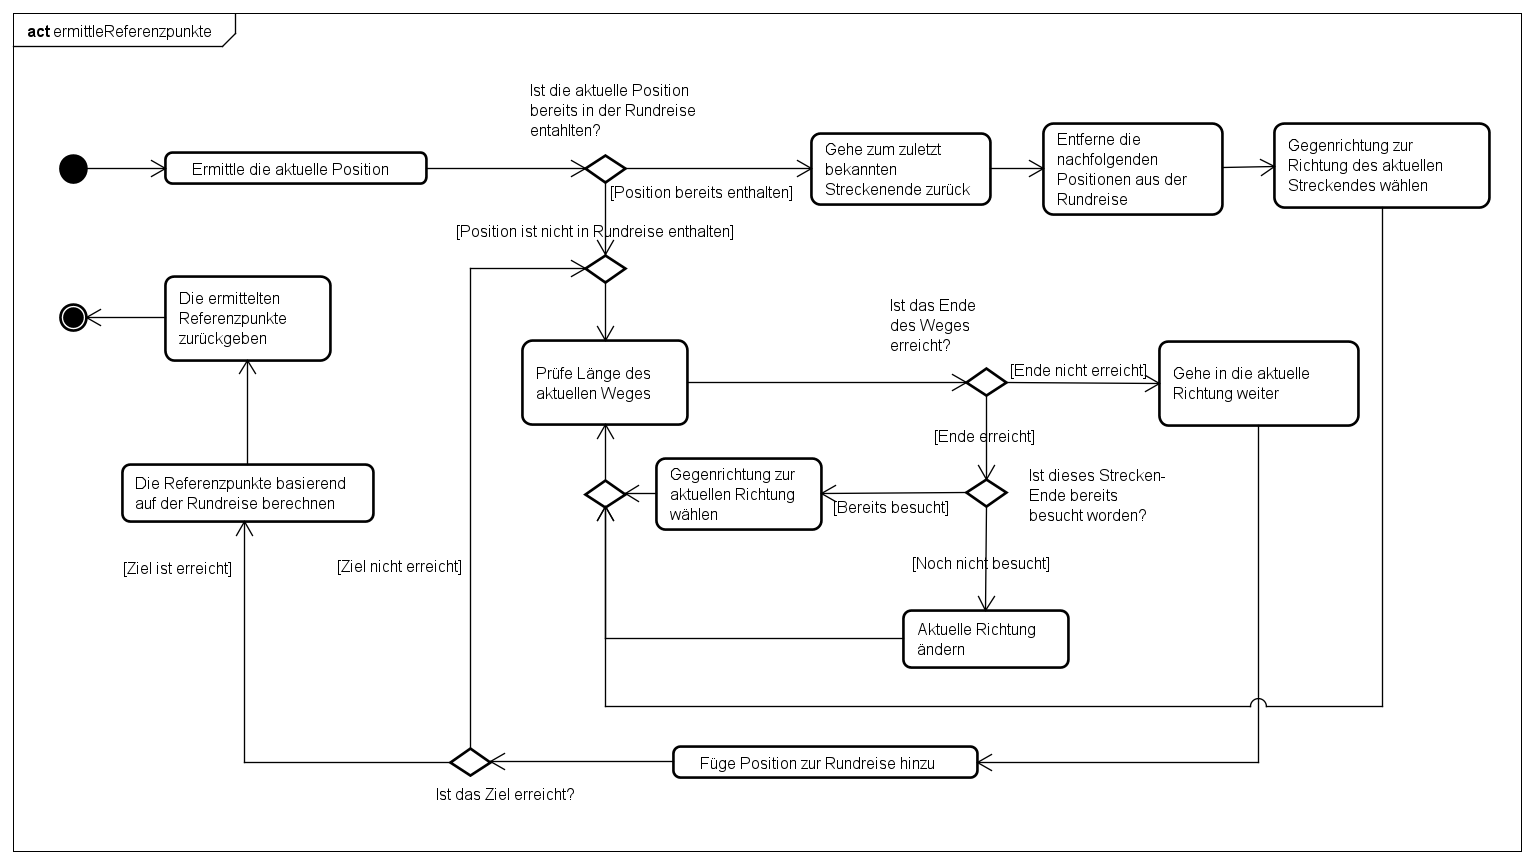
\includegraphics[scale=0.4]{pics/ermittleReferenzpunkte.png}
\caption{Ermittlung der Referenzpunkte}
\label{fig:aktivity_refp}
\end{figure}

\autoref{en-pkt1} prüft lediglich die Länge der aktuellen Fahrbahn bis zum Ende. Solange man sich auf einem akzeptierten Weg (z.B. Asphalt) befindet, wird in die aktuelle Richtung weitergegangen und diese Position wird zur Ergebnisstrecke, die den Weg von Ausgangsposition bis Ziel beschreibt, aufgenommen.\\
Ist das Streckenende erreicht, so wird mit \autoref{en-pkt2} die nächste Fahrtrichtung ermittelt. Da hier lediglich die Richtungen \glqq links\grqq{}, \glqq rechts\grqq{}, \glqq oben\grqq{} und \glqq unten\grqq{} berücksichtigt werden, ergeben sich folgende Fälle:
\begin{itemize}
\item Die ursprüngliche Richtung ist \glqq oben\grqq{} oder \glqq unten\grqq{}: Es kann lediglich nach \glqq links\grqq{} oder \glqq rechts\grqq{} weitergefahren werden, da der Algorithmus bereits aus der Gegenrichtung (z.B. ist bei \glqq oben\grqq{} die Gegenrichtung \glqq unten\grqq{}) gekommen ist.
\item Die ursprüngliche Richtung ist \glqq links\grqq{} oder \glqq rechts\grqq{}: Es kann lediglich nach \glqq oben\grqq{} oder \glqq unten\grqq{} weitergefahren werden.
\end{itemize}
Ist also der Algorithmus auf ein Straßenende gestoßen, so wird lediglich die Richtung gewechselt und \autoref{en-pkt1} wird fortgeführt.\\
Trifft der Algorithmus auf eine Ecke und entscheidet sich zuerst für die Richtung, in die nicht weitergegangen werden kann, so ist \autoref{en-pkt3} notwendig. Hierbei werden zusätzlich alle bereits erreichten Streckenenden gespeichert. Wird also ein Ende erreicht, das bereits besucht wurde, so wird in die Gegenrichtung zur aktuellen Richtung weitergefahren. Befindet sich also beispielsweise die aktuelle Position in einer Ecke, bei der man nach \glqq oben\grqq{} weiterfahren soll, der Algorithmus entscheidet sich jedoch zuerst nach \glqq unten\grqq{} weiterzufahren, so wird in diesem Fall, da die Ecke bereits einmal behandelt wurde, nach \glqq oben\grqq{} weitergefahren (nachdem zuvor die Strecke nach \glqq unten\grqq{} betrachtet wurde).\\
Als weiteren Mechanismus ist es notwendig auf bereits erreichte Positionen zu prüfen, da dies bedeuten würde, dass der Algorithmus einmal im Kreis gelaufen ist. In so einem Fall wird der aktuelle Weg solange zurückgelaufen, bis das zuletzt erreichte Straßenende erreicht wurde. Hierbei werden diese Positionen auch aus der Ergebnisstrecke entfernt. Ist das zuletzt bekannte Straßenende erreicht, so wird in die Gegenrichtung dieser Ecke weitergegangen. Mithilfe dieses Mechanismus wird der Kreis verlassen.\\
Ist das Zielfeld erreicht und somit ein Ringschluss gefunden worden, erfolgt \autoref{en-pkt4}. Hierbei gibt der Nutzer die Anzahl an zu verwendenden Referenzpunkten vor. Es wird die Ergebnisstrecke in diese Anzahl aufgeteilt und das jeweilige Sub-Streckenende wird als Referenzpunkt gewählt.\\
Somit ist der Algorithmus zur Berechnung der Referenzpunkte anhand des kompletten Spielfeldes ausführlich erläutert worden. Anschließend wird auf eine KI-ähnelnde Version desselben Algorithmus eingegangen.

\subsubsection{Berechnung der Referenzpunkte innerhalb eines vorgegebenen Radius}
Die Grundidee dieser Version ist ähnlich des zuvor erläuterten Algorithmus. Hier wird lediglich ein zusätzlicher Zähler eingesetzt, der auf den angegebenen Sicht-Radius überprüft. Dieser Zähler erhöht sich, wenn der Algorithmus eine Kachel in die aktuelle Richtung weitergeht. Befindet sich der Algorithmus auf dem Rückweg, da beispielsweise eine Sackgasse erreicht wurde, so werden diese Kacheln von dem Zähler abgezogen, da nun ein anderer Teil des Umfelds betrachtet wird. Ist das Maximum, also der angegebene Radius, erreicht, so wird die aktuelle Kachel automatisch als Referenzpunkt gewählt. Will der Anwender nun den nächsten Referenzpunkt, so wird an dem zuletzt ermittelten Referenzpunkt fortgesetzt und der Prozess wiederholt sich. Zusätzlich werden alle bereits ermittelten Referenzpunkte abgespeichert.\\
Erreicht nun der Algorithmus einmal das Ziel der Rennstrecke, so wird nicht mehr nach den nächsten Referenzpunkten simuliert, sondern die gespeicherten Referenzpunkte werden lediglich ausgegeben. Dies soll das Wissen der KI repräsentieren, dass der Algorithmus bei der Berechnung angesammelt hat.

\subsection{Die triviale KI}
Um die bereits genannten KI-Algorithmen mit einem Basisalgorithmus zu vergleichen, wird eine \textit{triviale KI} eingeführt. Das Ziel dieses Algorithmus ist es lediglich mehrere Runden des Rennens zu schaffen. Auf weitere Optimierungen wird dabei verzichtet, um die Intelligenz des Algorithmus so niedrig wie möglich zu halten. Es wird also lediglich die Rennstrecke abgefahren und erst bei Erreichen eines Straßenendes der nächste Weg ermittelt. Wird das Auto aufgrund der Zentrifugalkraft oder aufgrund eines anderen Spielers von der Rennstrecke abgebracht, so soll die triviale KI wieder auf den zuletzt bekannten Punkt der Rennstrecke fahren und anschließend den ursprünglichen Weg fortsetzen. Zusätzlich wird ein Mechanismus benötigt, der beim Erreichen eines Straßenendes trotzdem die Weiterreise des Algorithmus ermöglicht.\\
Die triviale KI akzeptiert hierbei Kacheln, die eine gerade Strecke, das Ziel oder die Startpositionen darstellen. Diese Kacheln werden im folgenden als akzeptierte Kacheln bezeichnet. Um nicht von der Strecke abzukommen werden Übergangskacheln zwischen beispielsweise Grass und Weg, Kurven und Grass nicht akzeptiert und als nicht akzeptierte Kacheln bezeichnet.\\
Der Algorithmus wiederholt hierbei folgende Schritte, bis das Spielende erreicht ist:
\begin{enumerate}
	\item Überprüfung, ob das eigene Auto von einer akzeptierten Kachel abgekommen ist. Ggf. wird die Fahrtrichtung in Richtung der zuletzt akzeptierten Position angepasst,
	\item Überprüfung, ob die aktuelle Fahrtrichtung beibehalten werden kann. Ggf. wird die nächste Fahrtrichtung ermittelt und in diese gelenkt.
	\item Fahre in die aktuell ermittelte Richtung weiter. 
\end{enumerate}

\begin{figure} [h]
\centering
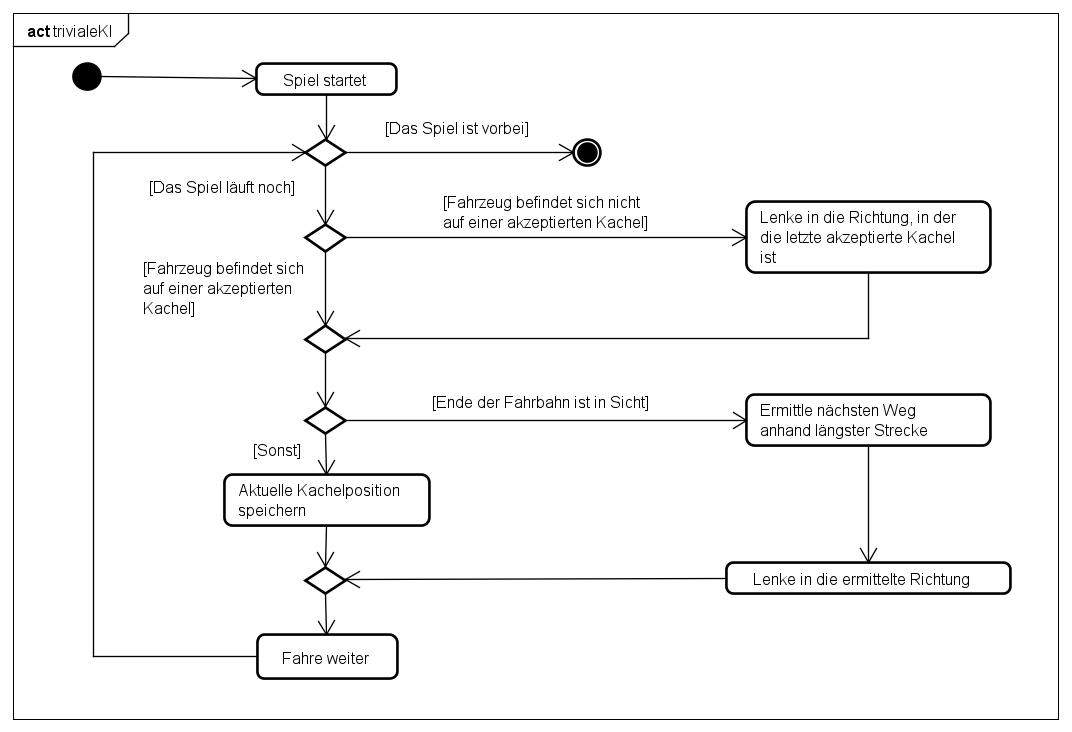
\includegraphics[scale=0.5]{pics/aktivitaet_trivialeKI.png}
\caption{Implementierung der trivialen KI}
\label{fig:trivialeKI}
\end{figure}

Wie in \autoref{fig:trivialeKI} dargestellt, prüft die triviale KI zuerst, ob die eigenen Koordinaten eine akzeptierte Kachel darstellt. Ist dies der Fall, so wird anschließend überprüft, ob sich in unmittelbarer Nähe eine nicht akzeptierte Kachel (z.B. eine Mauer oder eine Kurve) zu finden ist. Hierfür werden die zwei kommenden Kacheln in der aktuell gefahrenen Richtung betrachtet.\\
Die triviale KI verwendet hierbei die dynamische Version des Referenzpunkt-Algorithmus und fragt den nächsten Referenzpunkt erst ab, wenn der aktuelle erreicht ist. Hierbei überprüft der Algorithmus jede neue Kachel, die das Fahrzeug der trivialen KI erreicht. Stellt diese Kachel den aktuellen Referenzpunkt dar, so wird erst hier der nächste Punkt ermittelt. Die Fahrt fortgeführt.\\
Falls der akzeptierte Weg endet, wird ermittelt, in welche Richtung zu fahren ist. Hierbei werden die Richtungen betrachtet, die sich im 90° und -90° Winkel zur aktuellen Fahrtrichtung befinden. Beträgt die aktuelle Fahrtrichtung beispielsweise \glqq links\grqq{} so werden die Richtungen \glqq oben\grqq{} und \glqq unten\grqq{} betrachtet, wie in \autoref{subfig:richtung_vektor} zu sehen ist. Damit die triviale KI nicht in die Richtung fährt, aus der sie gekommen ist, orientiert sich der Algorithmus an die Koordinaten der Referenzpunkte, die regelmäßig ermittelt werden. Fährt das Auto beispielsweise nach links, so wird überprüft, ob sich der nächste Referenzpunkt oberhalb oder unterhalb der aktuellen Position befindet. Im Falle des Beispiels in \autoref{subfig:richtung_entscheidung} entscheidet sich die triviale KI für die Richtung \glqq oben\grqq{}, da sich der nächste Referenzpunkt oberhalb des Autos befindet.\\
\begin{figure}[h]
\centering
\begin{minipage}{0.45\textwidth}
\centering
	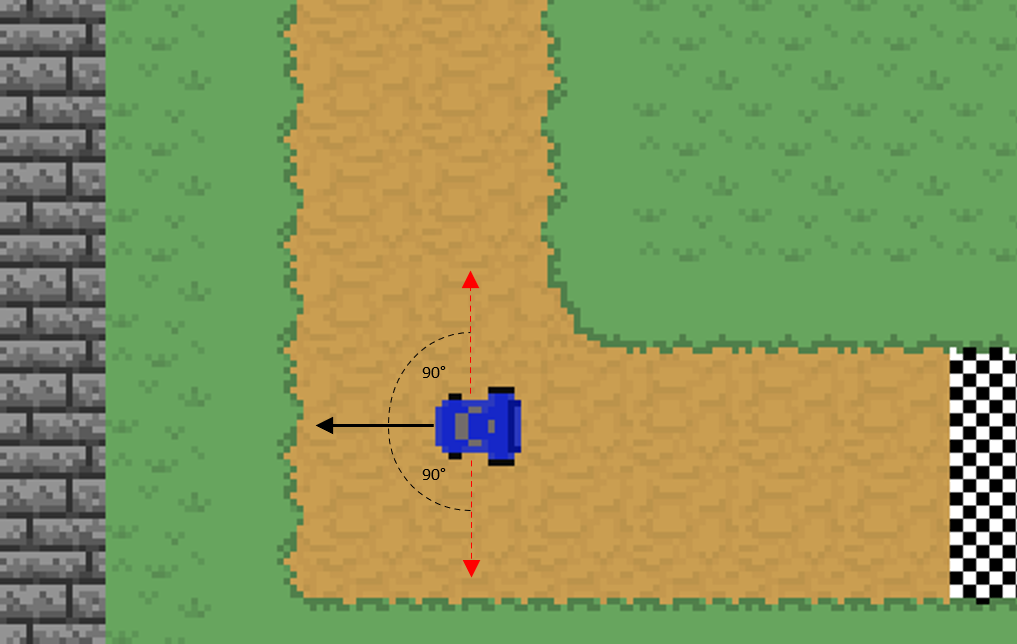
\includegraphics[scale=0.3]{pics/fahrtrichtung_vektor.png}
	\subcaption{Zu prüfende Richtungen}
	\label{subfig:richtung_vektor}
\end{minipage}
\qquad
\begin{minipage}{0.45\textwidth}
\centering
	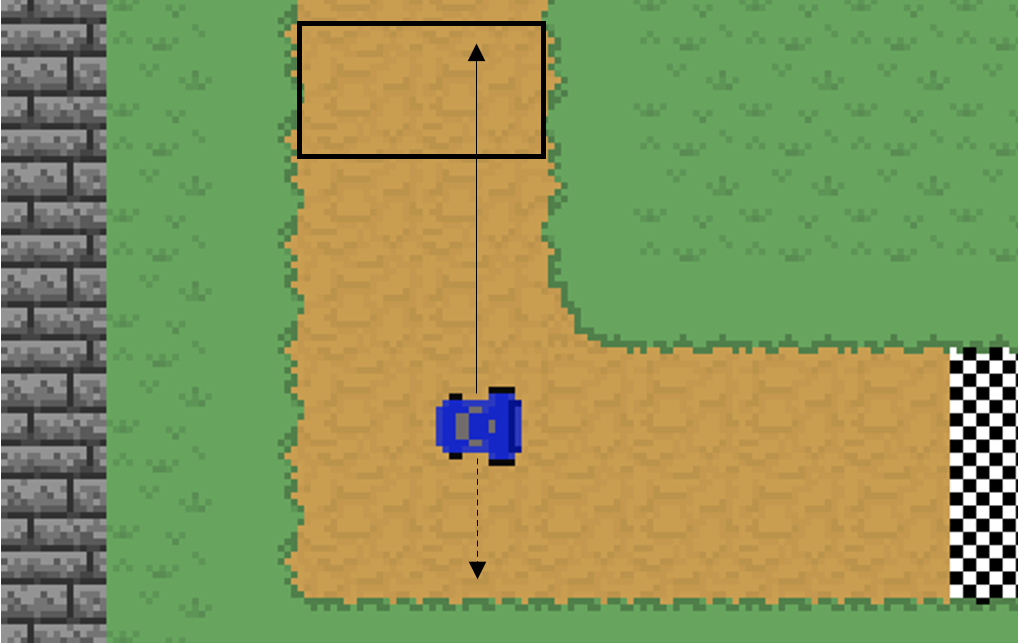
\includegraphics[scale=0.3]{pics/fahrtrichtung_entscheidung.png}
	\subcaption{Weg nach oben ist länger}
	\label{subfig:richtung_entscheidung}
\end{minipage}
\caption{Beispiel zur Richtungsentscheidung}
\label{fig:richtungsenscheidung}
\end{figure}

Befindet sich der Spieler andernfalls auf einer akzeptierten Kachel und mehr als zwei Folgekacheln stellen einen akzeptierten Weg dar, so wird die aktuelle Richtung beibehalten und die aktuelle Kachelposition wird gespeichert.\\
Die gespeicherte Kachel wird hierbei verwendet, um wieder auf die Fahrbahn zu gelangen, falls der Spieler von der Fahrbahn abgekommen ist. Dies kann auftreten, falls der Spieler von einem Gegner gerammt wird oder falls die Zentrifugalkraft den Spieler von der Fahrbahn abkommen lässt. Da die zuletzt gespeicherte Kachel eine akzeptierte Kachel darstellt, wird diese als Referenzpunkt verwendet und in deren Richtung gelenkt. Hat der Spieler die gespeicherte Kachel erreicht, so wird anschließend in die Richtung gelenkt, in welche die triviale KI ursprünglich fahren wollte.\\
Um zusätzlich einen Mechanismus anzubieten, der überprüft, ob die triviale KI gerade in die falsche Fahrtrichtung fährt, da beispielsweise die Kollision mit einem anderen Spieler das Auto verdreht hat, wird hierfür ein Zähler verwendet, der die Distanz zum nächsten Referenzpunkt darstellt. Mit jeder Kachel, die das Auto weiterfährt, wird dieser Zähler erhöht. Ist die angegebene Distanz, z.B. der vordefinierte Radius des Referenzpunkt-Algorithmus, erreicht, so wird vermutet, dass die triviale KI gerade in die falsche Richtung fährt. Als Gegenmaßnahme wird hierbei in die gegenteilige Fahrtrichtung gelenkt und der Zähler auf den Initialwert zurückgesetzt. Da sich nun die triviale KI weiter weg vom aktuellen Referenzpunkt befinden kann, wird der Distanzwert verdoppelt. Anschließend wird die Fahrt fortgesetzt.\\
Ist das Spielende erreicht, so wird der Algorithmus beendet.


\subsection{Implementierung der KI-Algorithmen}

Im Folgenden soll auf die Implementierung der KI-Algorithmen eingegangen werden.\newline
Dabei wird zunächst auch der zugehörige SpielGraph vorgestellt. Abschließend werden auch Anpassungesmöglichkeiten im Fahrverhalten der KI beleuchtet.

\subsubsection{Spielegraph}

Der Graph, den die Graphenalgorithmen für die Berechnungen der kürzesten Wege verwenden,
lässt sich schlicht auch als 2-dimensionales gefülltes Koordinatensystem betrachten.
Dabei stellen sämtliche X- und Y-Paare im definiertern Bereich einen Knoten (\textit{SpielKnoten}) dar.
Diese Knoten sind durch Kanten miteinander verbunden: Jeder Knoten besitzt 8 Nachbarknoten.(Siehe Abbildung drölf; bis auf die nahe dem Map-Rand gelegenen Knoten)
Initial bei Spielstart, werden sämtliche (600) \textit{SpielKnoten} initialisiert.
Während den Kalkulationen der Algorithmen können diese, nun zusammengefasst als eine Java-\textit{ArrayListe}, mit folgenden Attributen 
versehen werden:\newline
\textbf{NachbarKnoten}: Die 8 \textit{NachbarKnoten} ein\newline
\textbf{Direction}: Die Direction definiert ein Java-\textit{Enum}. Dort werd die Ausrichtung/Himmelsrichtung der \textit{NachbarKnoten} festgelegt.\newline
\textbf{kosten, heuristik, funktion, distanz}: Diese Attributee werden vom A-Stern-Algorithmus verwendet.
Deren Funktion und Nutzen werden in Abschnitt drölf genauer erläutert.\newline
\textbf{ElternKnoten}: (Im Code Refactorn!)\newline
\textbf{kiPfadElement}: für Ausgabe(Zeichnen) des KI-ermittelten Pfades in der (Acronym!)IDE-Konsole\newline
\textbf{gesehen}: Diese Membervariable wird vom Dijkstra-Algorithmus verwendet und daher im Abschnitt drölf beschrieben.\newline

Attribute und Funktionen, die für Graphen Algorithmen notwendig sind(Nachbarknoten,...)

\subsubsection{Abstract Class KI}

kurz Allgemein: Warum Abstrakte Klasse in Software Entwicklung und wie hier realisiert\newline
dann: Wie hier implementiert (in Java): Kein Interface, da manche Methoden von der ErbenKlasse implementiert werden sollen, allerdings nicht alle(später vielleicht nichtGraphAlogrithmen, die aber auch updateVoid dann für sich implementieren können und alle anderen Funktionen ggf übernehmen können)


Warum? Um weitere KI-Clients leicht implementieren zu können.(Gemeinsamkeiten können wiederverwendet werden) \newline
Außerdem: Freies Anpassen des Fahrverhaltens durch KI-Fahrverhalten(später im Kapitel)

Abschließend eine Grafik mit Übersicht

\subsubsection{A-Stern}

\subsubsection{Dijkstra}

evtl abschließend kurz Gemeinsamkeiten/Unterschiede der beiden

\subsubsection{Richtungsentscheidung}

1.Spielknoten des ermittelten Pfades\newline
erneutes Berechnen der Nachbarknoten\newline
dadurch Richtungsentscheidung WASD\newline
Grafik mit 3x3 Quadraten und den Richtungen\newline


\subsubsection{KI-Fahrverhalten}

\textbf{Entschleunigung vor Kurven}

\textbf{Umkehren nach Verlassen der Fahrban}

\textbf{Kollisionscheck}

\subsection{Implementierung der Ziele}

\section{Diskussion zu den Algorithmen}
\subsection{Diskussion zur trivialen KI}
Was die triviale KI betrifft, so ist sofort zu erkennen, dass sich das Auto des Algorithmus immer am äußeren Rand der Fahrbahn befindet. Zusätzlich wird das Fahrzeug in fast jeder Kurve aus der Fahrbahn geschleudert, da der Algorithmus nicht bremst. Der Mechanismus, der das Erkennen der Fahrt in die falsche Richtung erkennt, erfüllt seinen Zweck. Jedoch kann dies aufgrund einer hohen Wahl der Distanz zum nächsten Referenzpunkt ziemlich spät ausfallen. Der schlimmste Fall kann hierbei eintraten, wenn das Fahrtzeug in die Gegenrichtung fährt, wenn die aktuelle Kachel den vorherigen Referenzpunkt darstellt. So würde der Mechanismus hier erst eingreifen, wenn schon der vorletzte Referenzpunkt erreicht ist.\\
Eine weitere negative Eigenschaft der trivialen KI, ist das schlichte Fahren, ohne den kürzesten Weg zum nächsten Referenzpunkt zu ermitteln. Dies würde zum Erkennen einer Fahrt entgegen der Fahrtrichtung beitragen.\\
Eine positive Eigenschaft der trivialen KI ist jedoch, dass der eigentliche Rechenaufwand hauptsächlich in der Berechnung des nächsten Referenzpunktes liegt, da lediglich die nächste Fahrtrichtung erst bei Erreichen eines Straßenendes erfolgt.\\
Da die triviale KI und der Algorithmus zum Berechnen der Referenzpunkte ähnlich beim Berechnen der Fahrtrichtung vorgehen, so hat dieser die ähnliche Vor- und Nachteile wie die triviale KI. Die Simulation zum nächsten Referenzpunkt erfolgt hierbei auch am äußeren Straßenrand.\\
Außerdem können die Algorithmen in deren aktuellen Umsetzung nicht auf eine Kreuzung reagieren, in der der Spieler beispielsweise von links kommt und nach oben oder unten weiterfahren soll.\\ 
Somit ergeben sich die folgenden Verbesserungsvorschläge für beide Algorithmen:
\begin{itemize}
\item Mithilfe eines Bremsmechanismus würde die triviale KI nicht mehr so oft von der Fahrbahn abweichen.
\item Würde Simulation des Referenzpunkte-Algorithmus im Inneren der Straße stattfinden, so würde der Sicht-Radius maximal ausgenutzt werden können. 
\item Bei Kreuzungen könnte der Mittelpunkt der Kreuzung zu den Randpunkten hinzugefügt werden, so würde bei einer Sackgasse zunächst dieser Punkt betrachtet werden.
\end{itemize}
Als Fazit lässt sich hierbei jedoch sofort ziehen, dass beide Algorithmen das Ziel, einen trivialen Algorithmus zum Bewältigen eines Rennspiels, erreichen. Hierbei ist es interessant die Algorithmen mit den genannten Verbesserungsvorschlägen zu erweitern und die Nachteile auszubessern.   

\pagebreak

\section{Vergleich OpenGL und Java-Swing}

\pagebreak

\section{Vergleich der Graphalgorithmen}
TODO: Zeitmessung im Code (von Funktionsaufruf bis zu Richtungsentscheidung)


http://www.hindex.org/2014/p520.pdf90
https://www.youtube.com/watch?v=g024lzsknDo
https://www.baeldung.com/cs/dijkstra-vs-a-pathfinding


\pagebreak
% ----------------------------------------------------------------------------------
% Kapitel: Fazit und Ausblick
% ----------------------------------------------------------------------------------
\section{Fazit und Ausblick}



\pagebreak

% ----------------------------------------------------------------------------------------------------------
% Filter fuer Literatur und Quellen definieren
% ----------------------------------------------------------------------------------------------------------

\defbibheading{Literatur}{\section*{Literaturverzeichnis}} 
\defbibheading{Quellen}{\section*{Quellenverzeichnis}} 
  
\defbibfilter{Literatur}{\not\keyword{online}} 
\defbibfilter{Quellen}{\keyword{online}} 


% ----------------------------------------------------------------------------------------------------------
% Literatur
% ----------------------------------------------------------------------------------------------------------
\lhead{} 
\rhead{Literaturverzeichnis} 

\printbibliography[heading=Literatur,filter=Literatur] 

\pagebreak


% ---------------------------------------------------------------------------------------------------------- 
% Quellen 
% ---------------------------------------------------------------------------------------------------------- 
\lhead{} 
\rhead{Quellenverzeichnis} 

\printbibliography[title = {Quellenverzeichnis}, heading=Quellen,filter=Quellen] 

\pagebreak 

% ----------------------------------------------------------------------------------------------------------
% Anhang
% ----------------------------------------------------------------------------------------------------------
\pagenumbering{Roman}
\setcounter{page}{1}
\lhead{Anhang \thesection}

\begin{appendix}
\section*{Anhang}
\phantomsection
\addcontentsline{toc}{section}{Anhang}
\addtocontents{toc}{\vspace{-0.5em}}



\section{Domänenmodell des Map-Editors}
In der folgenden Abbildung ist das Domänenmodell des Map-Editors dargestellt. Hier sind die Klassen in die Schichten Model, View und Controller aufgeteilt. Die Kommunikation zwischen der View- und der Model-Schicht erfolgt ausschließlich über die Controller-Schicht. Zusätzlich ist das Memento-Entwurfsmuster in der Controller-Schicht zu sehen.

\begin{figure}[h]
\centering
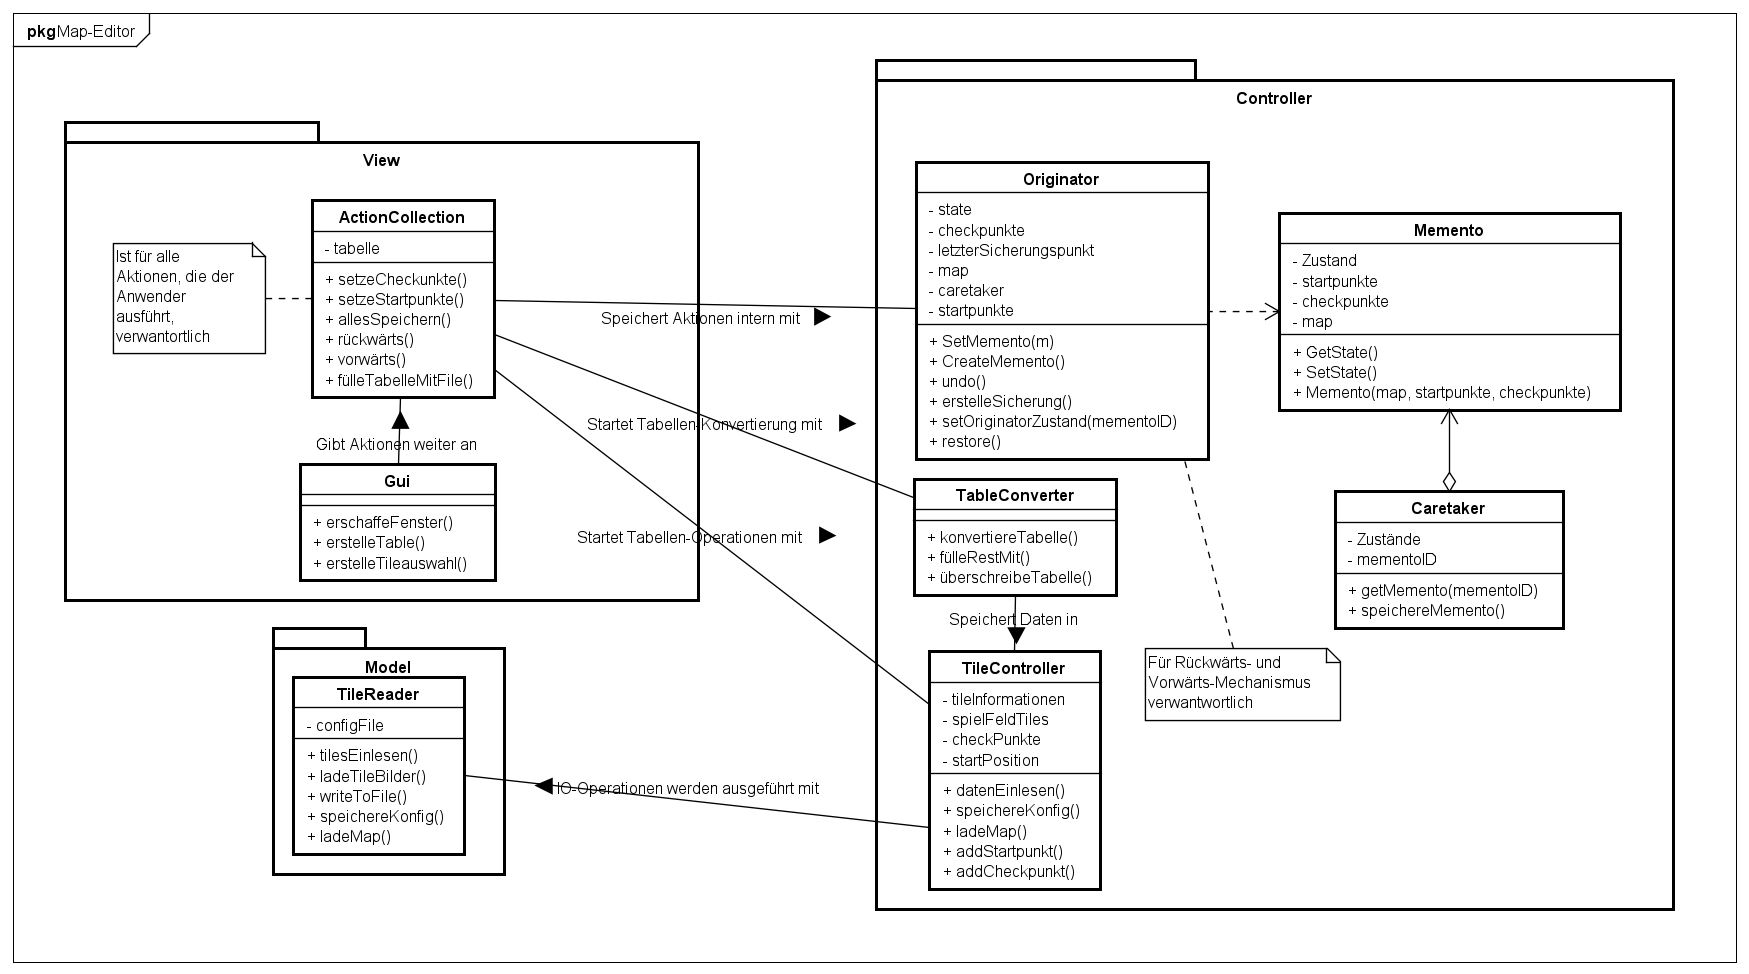
\includegraphics[width=\textwidth,keepaspectratio]{pics/domainmodell_mapeditor_complete.png}
%\caption{Domänenmodell}
\caption{Domänenmodell des Map-Editors}
\label{abb:domainmodell-mapeditor-complete}
\end{figure}


\end{appendix}


\pagebreak




\end{document}
